\part{Envisager la division sociale et sexuée du travail à partir des annonces: l'apport du \textit{topic modeling}}


\chapter{L'échec du LDA (\textit{Latent Dirichlet Allocation})}


Le \textit{topic modeling} est une méthode d'apprentissage non-supervisé qui emploie un modèle de probabilité pour associer des textes ou des parties de textes à des thèmes, ou \textit{topics}. Dans les faits, le \textit{topic model} va effectuer une opération de \textit{clustering}, c'est-à-dire tenter de rapprocher certains mots du corpus entre eux, en se basant sur leur similarité sémantique supposée. 

Appliqué au corpus de petites annonces, le \textit{topic modeling} peut être un moyen d'étoffer et de proposer un regard complémentaire et englobant aux incursions très localisées qui ont été faites jusqu'ici. 

\section{Méthode}


Le premier algorithme de \textit{topic modeling} que j'ai essayé d'appliquer au corpus est le LDA, ou \textit{Latent Dirichlet Allocation}, via la librairie python Gensim\footnote{Le site et la documentation de la librairie: \url{https://radimrehurek.com/gensim/}}. Le LDA est un modèle statistique qui repose sur l'hypothèse que chaque mot du corpus peut être associé à un \textit{topic}, en se basant sur la co-occurrence des mots au sein du corpus, considéré comme un sac de mots.

Le LDA s'applique donc sur un texte lemmatisé et sans stopwords, puisqu'il considère que chaque mot du corpus peut être associé à un \textit{topic} et possède donc une valeur sémantique définie. L'une des grandes différences entre le LDA et d'autres méthodes de \textit{topic modeling} est que les modèles de LDA nécessitent qu'on leur précise le nombre de \textit{topics} à générer. Dans le cas des annonces, j'ai ainsi pu tester l'algorithme de gensim et comparer les scores de performance du modèle en fonction du nombre de \textit{topics} générés. 

 

\section{Des résultats peu significatifs pour notre corpus}

Gensim génère deux scores de performance différents: la perplexité du modèle d'un côté, et sa cohérence de l'autre. La perplexité est une mesure de la surprise du modèle face à des données inédites, qu'il n'a jamais vues. En d'autres termes, une mesure d'à quel point de nouvelles données sont probables ou attendues étant donné les données que le modèle a déjà ingérées. Plus ce score est bas, moins le modèle a de chances d'être "surpris", et donc meilleur il est. Cependant, la perplexité en tant que score de performance a des limites, la première étant qu'elle est souvent décorrélée du jugement humain sur ce qui constitue un \textit{topic} pertinent ou non; en d'autres termes, elle n'est pas facilement interprétable\footcites{changReadingTeaLeaves2009}.  La cohérence du modèle, quant à elle, représente la similarité sémantique entre les mots au sein d'un \textit{topic}; elle est donc plus utile pour estimer l'efficacité réelle d'un modèle. On considère qu'un bon score de cohérence est compris entre 0.5 et 0.7. 

\begin{table}[ht]
	\centering
	\begin{tabular}{ccc}
		\hline
		\textbf{Topics} & \textbf{Cohérence} & \textbf{Perplexité} \\ \hline
		10                        & 0.37                        & -7.94                        \\
		20                        & 0.4                         & -15.01                       \\
		30                        & 0.39                        & -18.88                       \\
		40                        & 0.41                        & -22.73                       \\
		50                        & 0.4                         & -26.59                       \\
		60                        & 0.4                         & -30.59                       \\
		70                        & 0.39                        & -34.45                       \\
		80                        & 0.39                        & -38.41                       \\
		90                        & 0.39                        & -42.28                       \\ 
		100                       & 0.38                        & -46.28                       \\ \hline
	\end{tabular}
	\caption{Scores de performance du modèle en fonction du nombre de topics générés}
\end{table}

Néanmoins, avec un corpus nettoyé au préalable, on observe que la cohérence du modèle appliqué aux petites annonces ne dépasse jamais 0.41. L'examen des 40 thèmes générés par ce modèle met en évidence les difficultés du LDA sur ce corpus: les cinq premiers \textit{topics} contiennent des mots très rares dans le corpus, dont certains ont même plutôt l'air de résulter d'erreurs d'océrisation ou de segmentation des annonces. Les \textit{topics} suivants sont déjà plus cohérents (topic 7 sur les compétences féminines et manuelles, topic 8 sur les éléments de langage qui caractérisent l'annonce: placer, adresser, écrire, demande...) mais peuvent aussi présenter des redondances.

Ainsi, l'emploi du LDA et de gensim ne s'est pas révélé probant pour ce corpus. Plusieurs raisons pourraient expliquer cela: la longueur limitée des documents (bien qu'une découpe tous les 500 mots n'ait pas donnée de meilleurs scores qu'une découpe par annonce), la présence d'\textit{outliers} et d'anomalies qui rendent difficile une généralisation du modèle. 

\begin{figure}[ht]
	\centering
	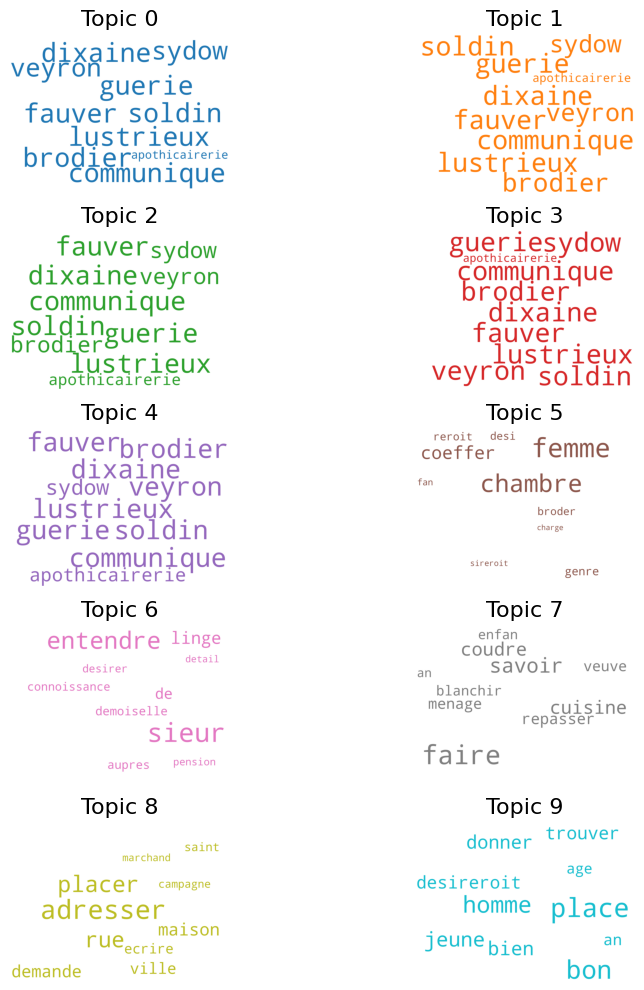
\includegraphics[width=12cm]{wordcloud_LDA.png}
	\caption{Nuage de mots des dix premiers topics du modèle}
\end{figure}




\chapter{Cartographier les frontières du travail et des annonces avec Top2Vec}

\section{Méthode}

Un second ensemble de \textit{topic models} repose cette fois non pas sur la co-occurrence de mots mais sur des \textit{embeddings}, c'est-à-dire une représentation vectorisée des mots du corpus et de leurs relations sémantiques. La première librairie que j'ai utilisée est Top2Vec, dont le fonctionnement est décrit de la manière suivante par ses créateurs: "L'algorithme postule que des documents similaires sémantiquement sont indicateurs d'un topic sous-jacent. La première étape est de créer un \textit{embeddin}g de document et de vecteurs de mots. Une fois les documents et les mots représentés dans un espace vectoriel, le but de l'algorithme est de trouver les amas les plus denses de documents, puis d'identifier quels mots ont attiré ces documents les uns vers les autres. Chaque amas est un topic, et les mots qui ont attiré les documents vers cet amas sont les mots appartenant au topic.\footnote{Description disponible sur le github de Top2Vec: \url{https://github.com/ddangelov/Top2Vec}}".
Ainsi, à l'inverse de Gensim, Top2Vec ne nécessite pas qu'on lui fournisse un nombre de\textit{ topics} prédéfinis, ni qu'on lemmatise ou nettoie de quelconque façon le corpus avant de le donner au modèle. L'un des seuls paramètres qu'on peut lui fournir au moment de la génération des \textit{embeddings} puis des \textit{topics} est la vitesse d'apprentissage (j'ai ici utilisé l'option "deep-learn", la plus lente mais qui fournit en théorie des résultats plus cohérents). Néanmoins, une fois les \textit{topics} générés, de nombreux traitements sont possibles.

Top2Vec appliqué au corpus des \textit{Affiches} génère 24 topics, que pour beaucoup on peut interpréter comme révélant un aspect ou une dimension des petites annonces d'emploi, qu'elle soit relative à l'économie de l'annonce, à la division et à la description du travail, voire même aux limites intrinsèques au corpus. 


\section{Économie de l'annonce}

Tout d'abord, plusieurs \textit{topics} générés par Top2Vec ont pour objet des éléments distinctifs des petites annonces, notamment les phénomènes d'adressage et d'intermédiation, visibles dans les topics 14 et 20 avec des mots comme "recevra", "ad(resser)", "lettres", "renseignemens". Les marques de la mise en valeur de soi sont également rendues visibles par le topic 21, qui met en avant les valeurs centrales que représentent l'honnêteté et la fidélité dans l'\textit{ethos} domestique.

\begin{figure}[ht]
	\centering
	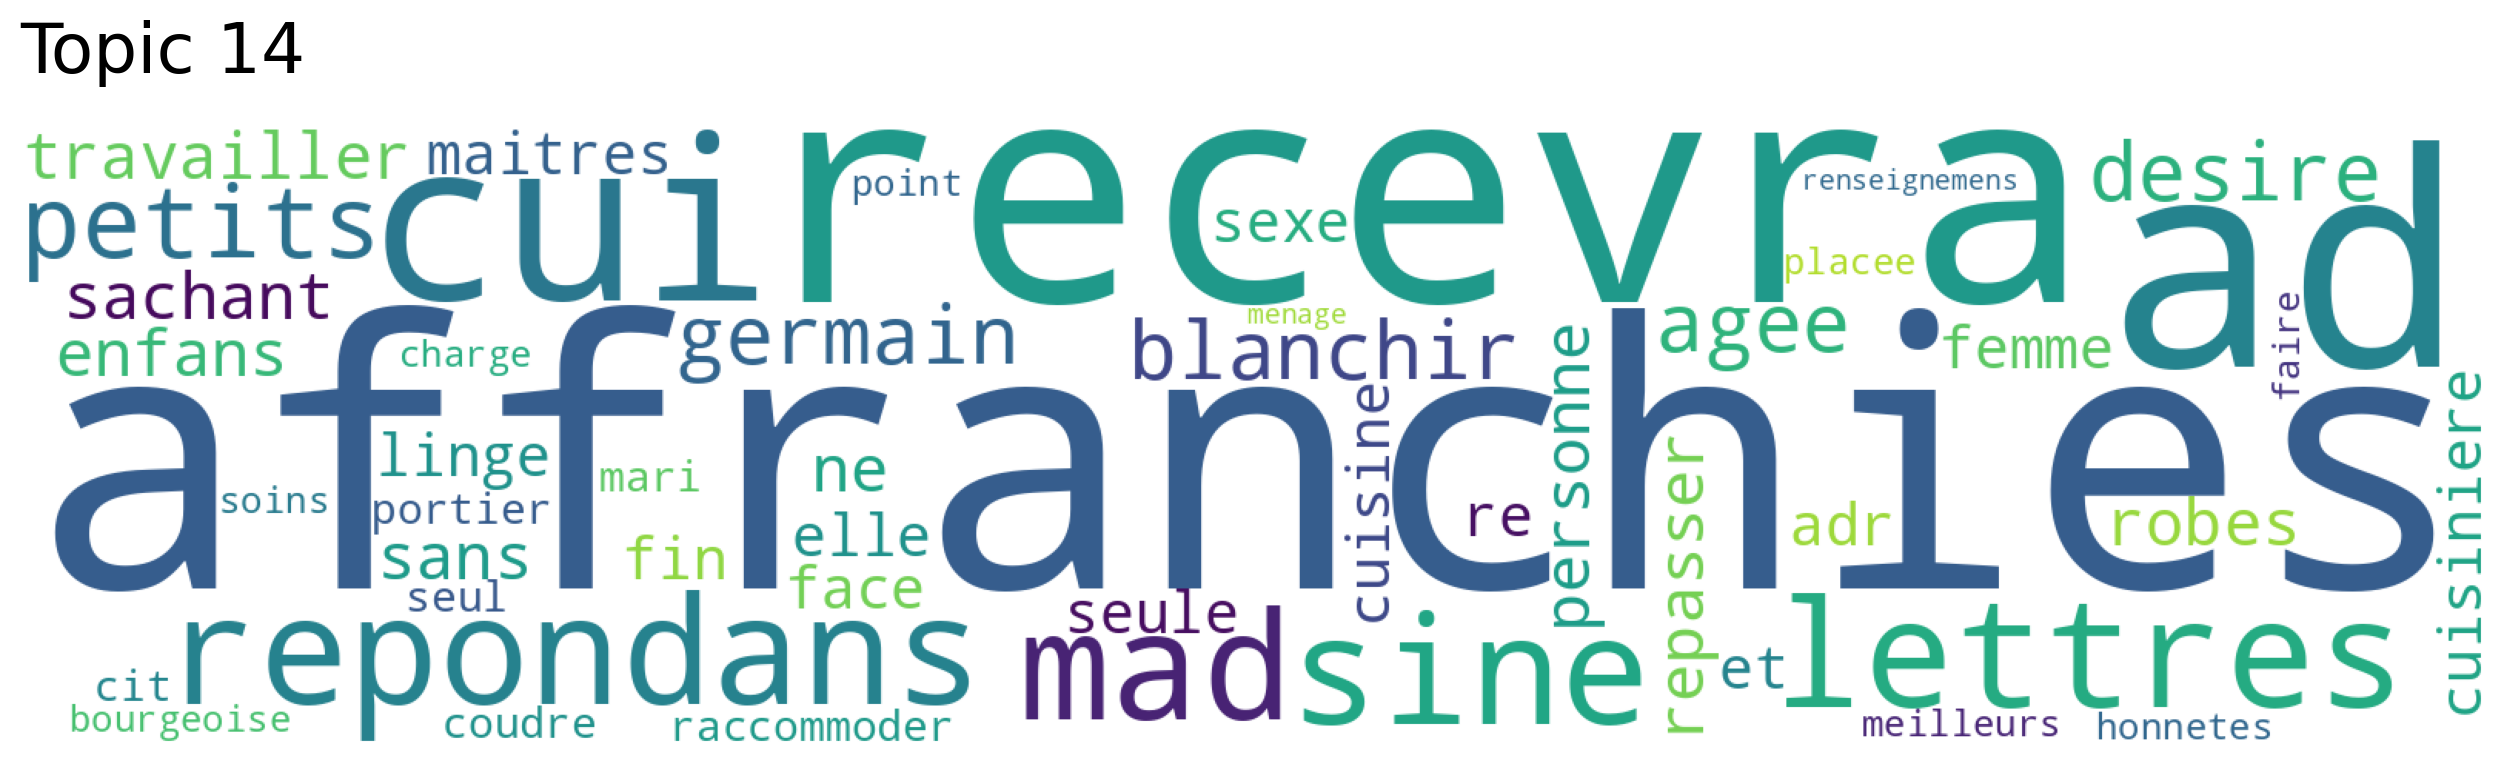
\includegraphics[width=12cm]{wordcloud_top2vec_14.png}
	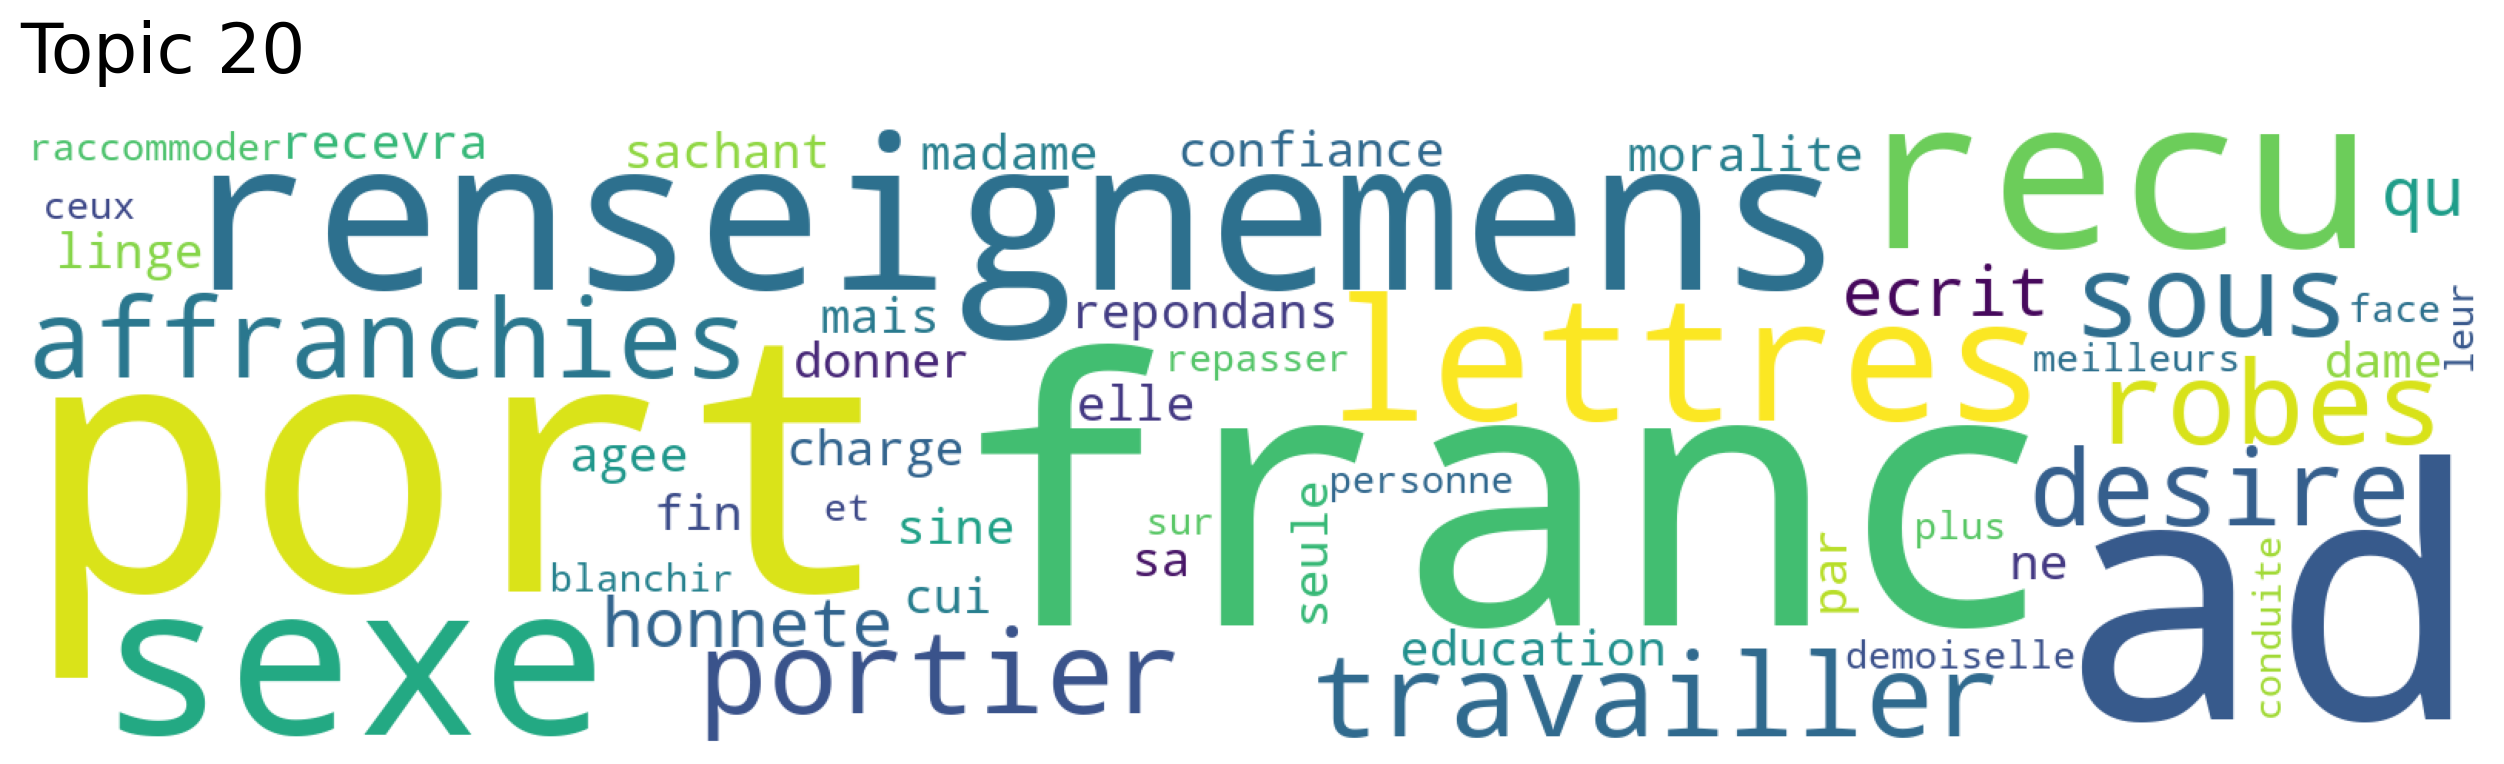
\includegraphics[width=12cm]{wordcloud_top2vec_20.png}
	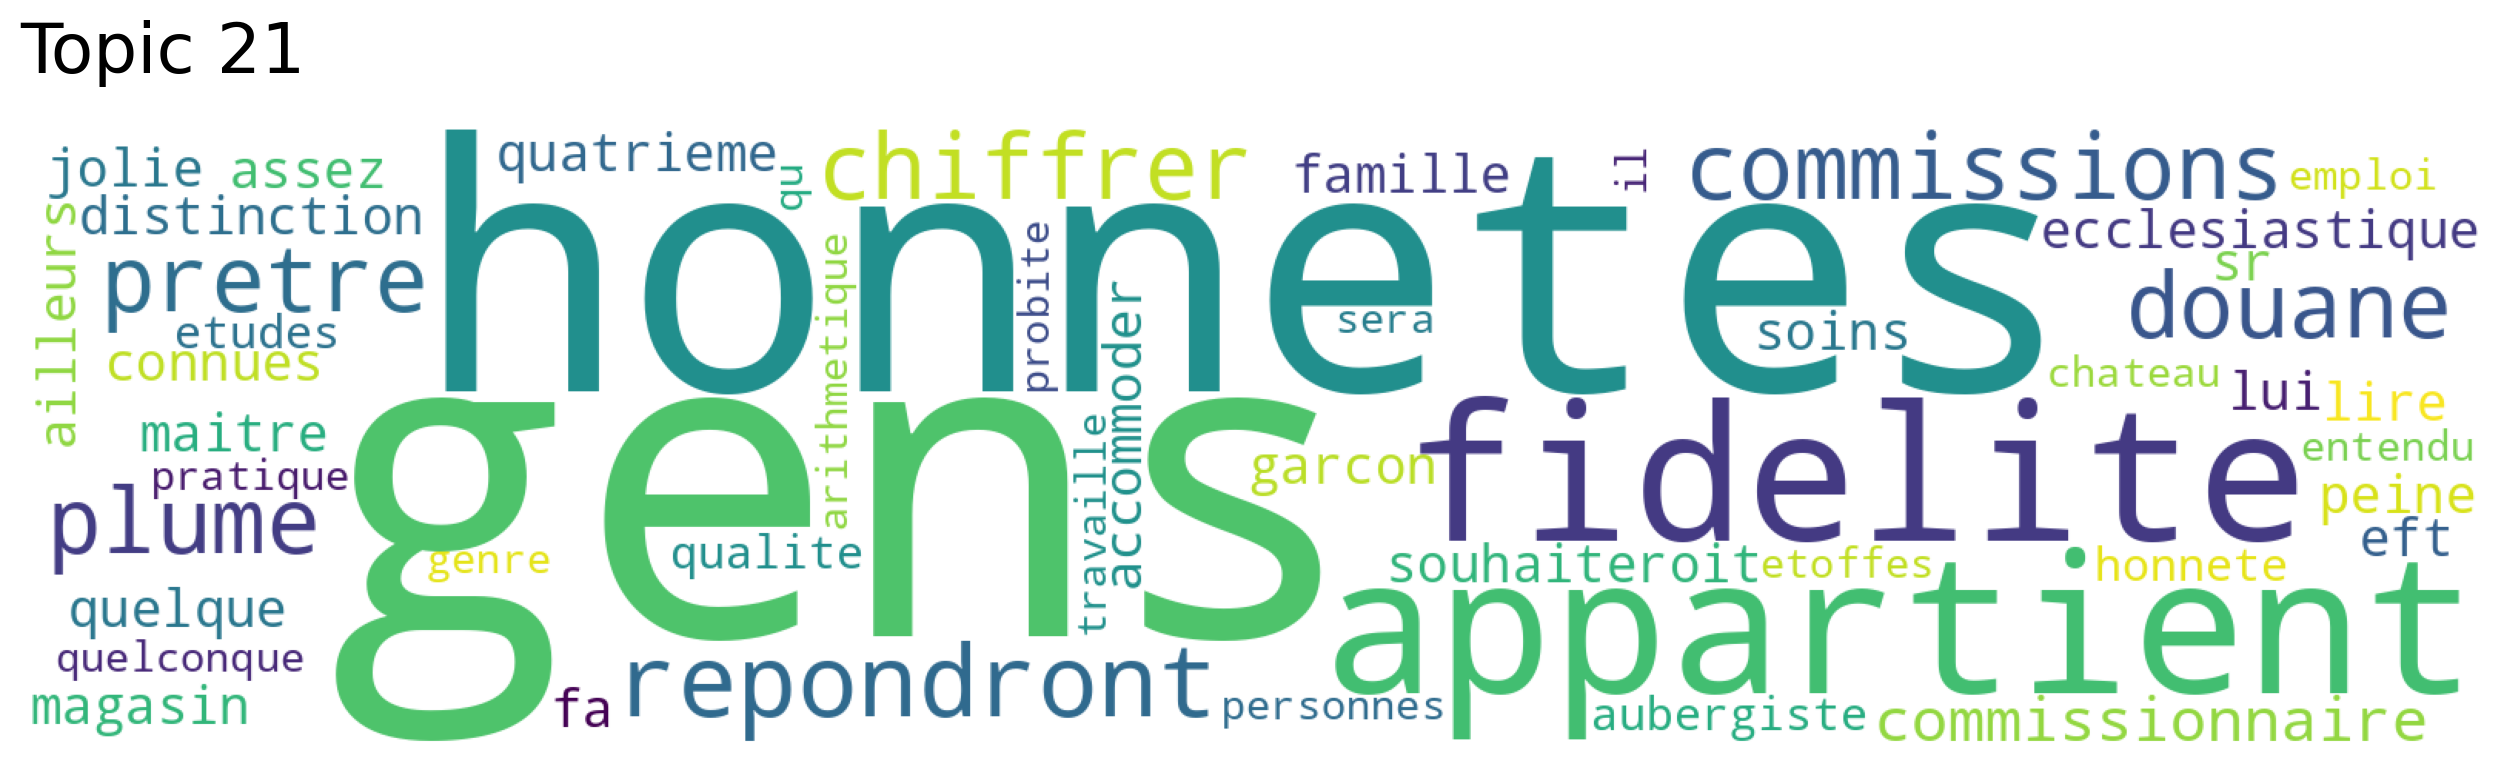
\includegraphics[width=12cm]{wordcloud_top2vec_21.png}
	\caption{Nuage de mots des topics 14, 20 et 21}
\end{figure}

\section{Des \textit{topics} genrés...}

Une deuxième observation qui peut être faite, et qui corrobore ce qu'on a déjà vu au chapitre 7, est celle d'une division fortement sexuée du travail domestique, rendue manifeste à travers la distinction par l'algorithme des compétences selon le sexe. D'un côté, les topics 0, 1 et 3 (qui comptent par ailleurs parmi les topics les plus importants du modèle) se rapportent plutôt aux travaux féminins, que ce soit à travers des qualificatifs de genre (fille, dame, veuve, citoyenne), des qualificatifs d'emplois ou de places (gouvernante) ou des verbes de compétences (raccommoder, cuisiner, blanchir, repasser). À l'inverse, les topics 2, 9 et 12 se rapportent plutôt à la domesticité masculine, encore une fois à travers des noms (garçon), des adjectifs (robuste) et des verbes (raser, panser, conduire, coiffer). 


\begin{figure}[h!t]
	\centering
	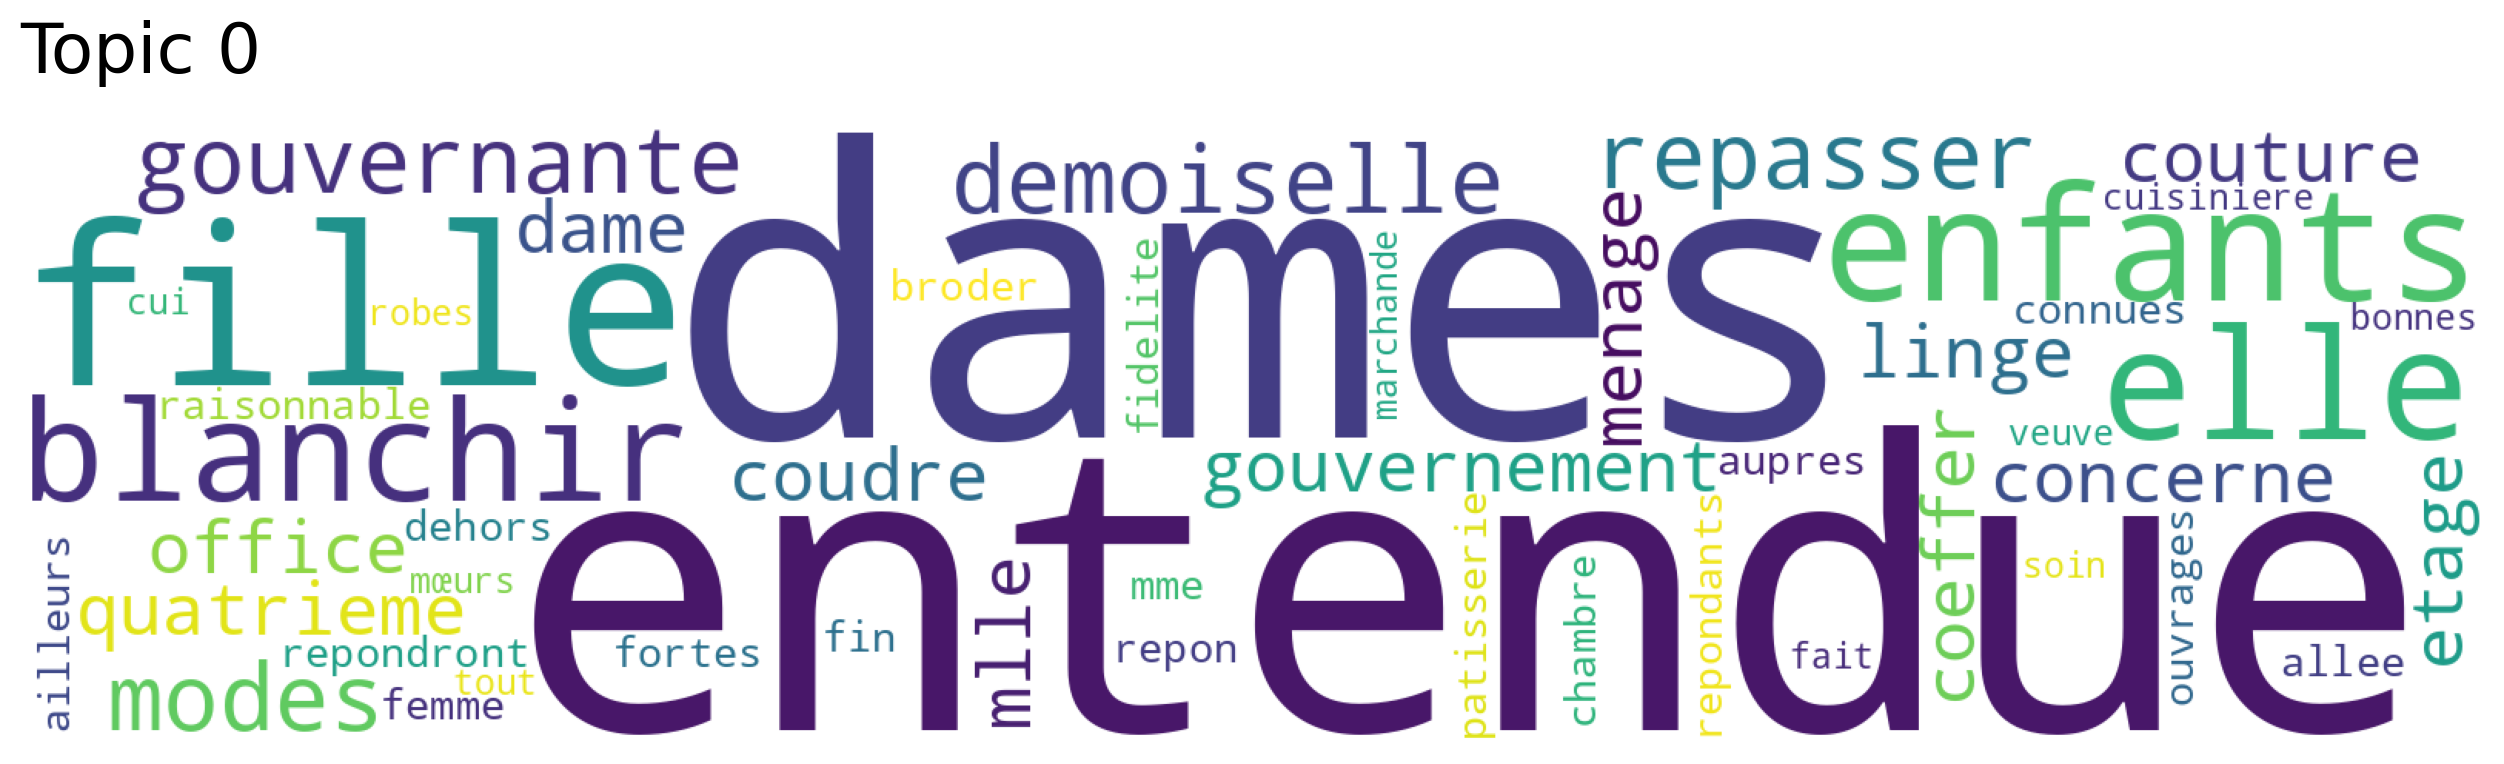
\includegraphics[width=12cm]{wordcloud_top2vec_0.png}
	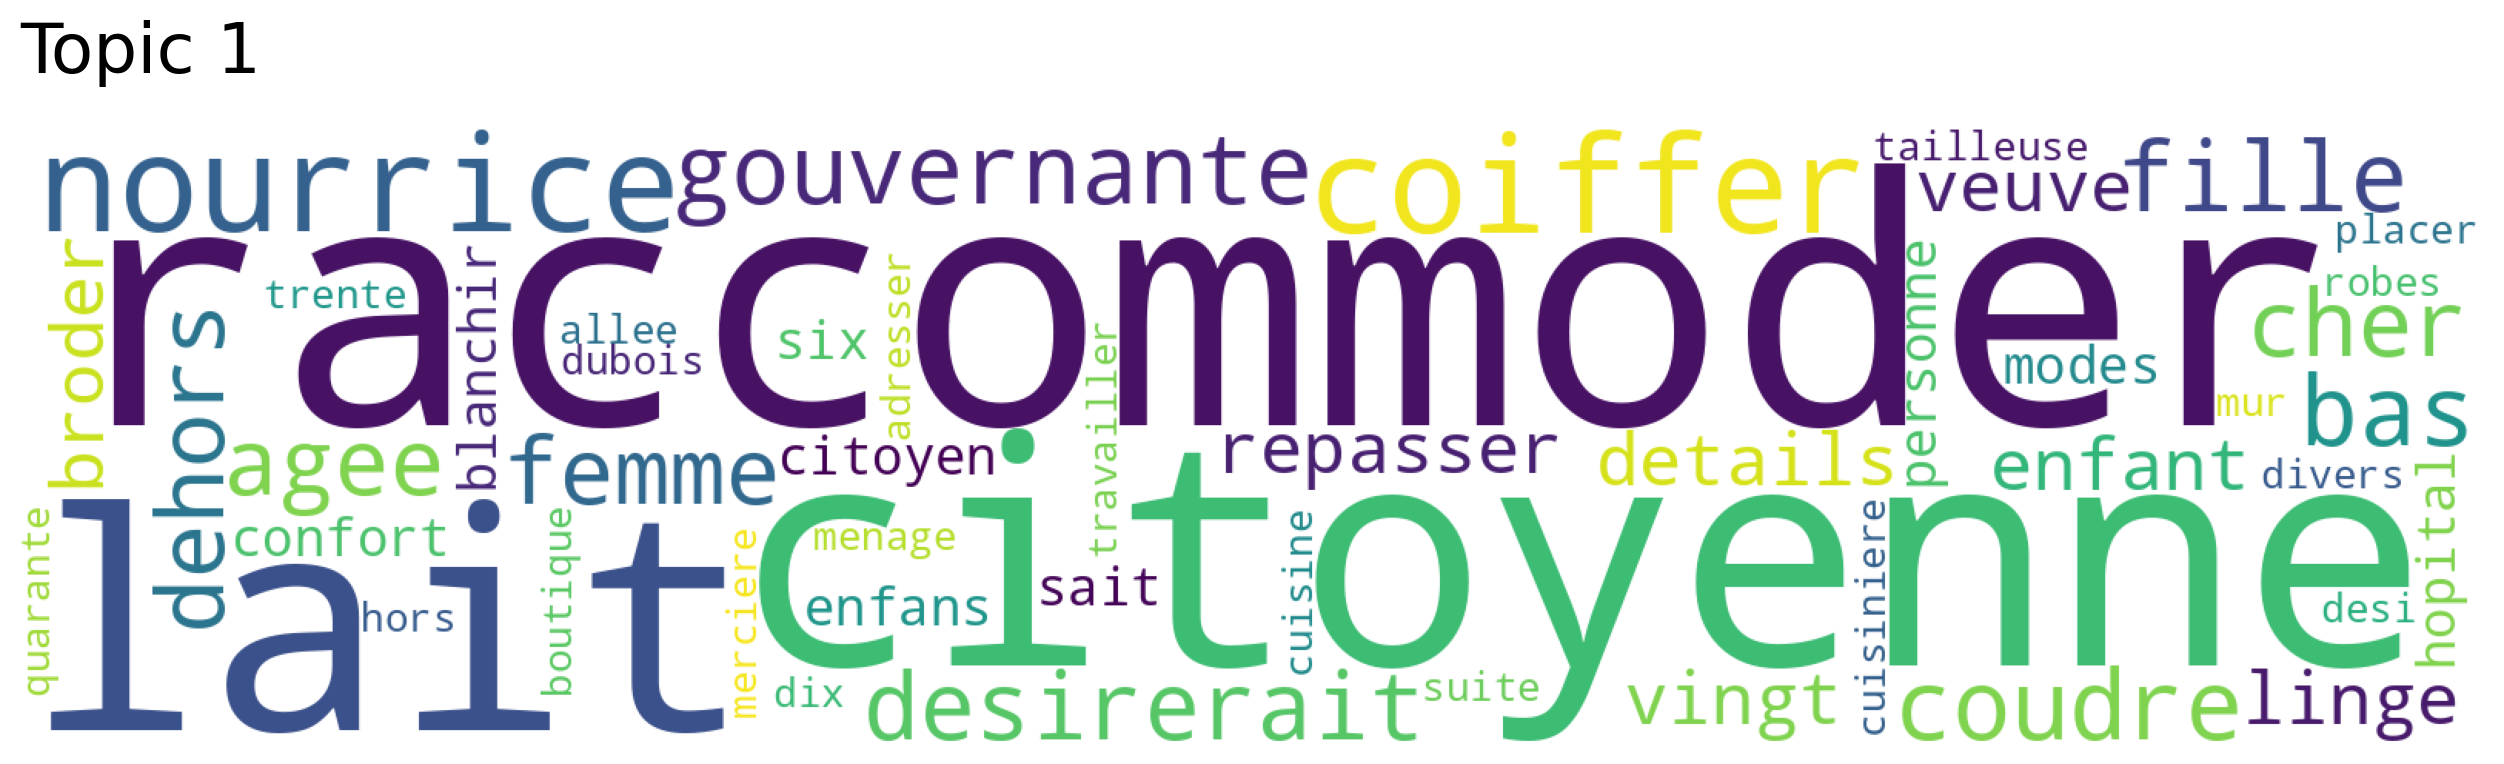
\includegraphics[width=12cm]{wordcloud_top2vec_1.png}
	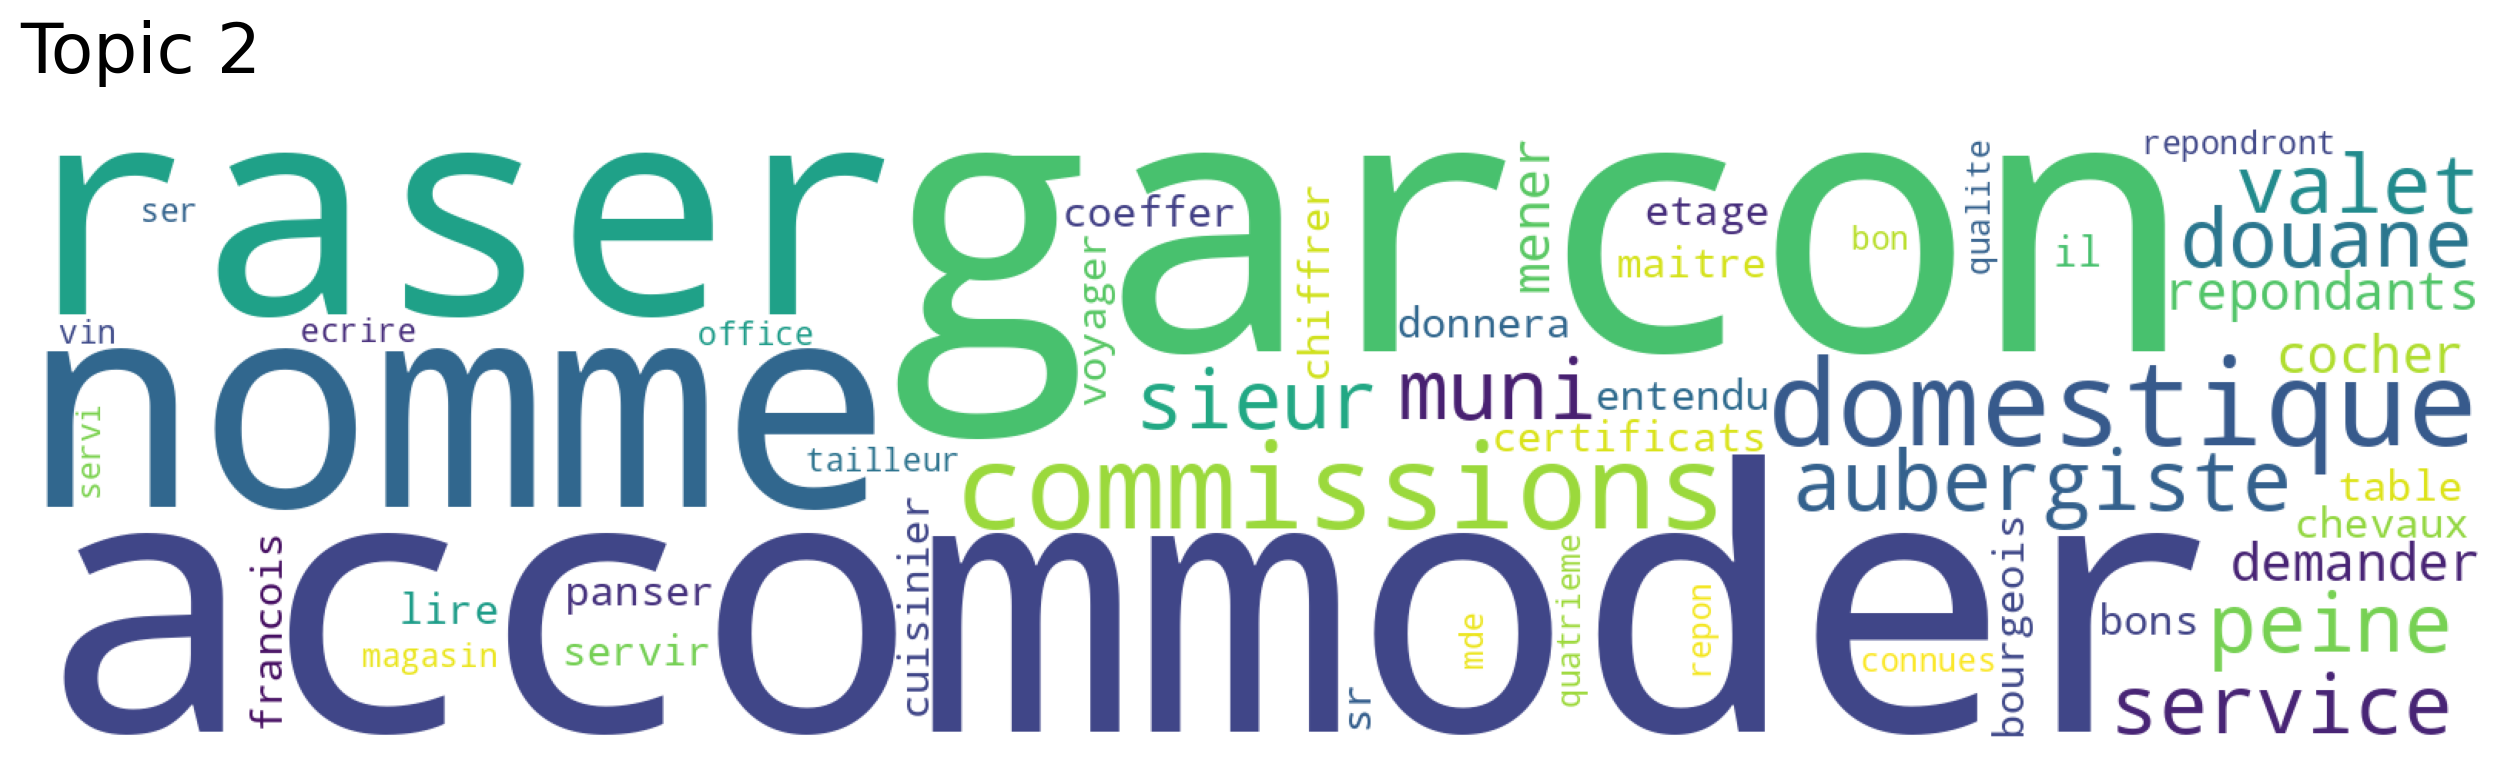
\includegraphics[width=12cm]{wordcloud_top2vec_2.png}
	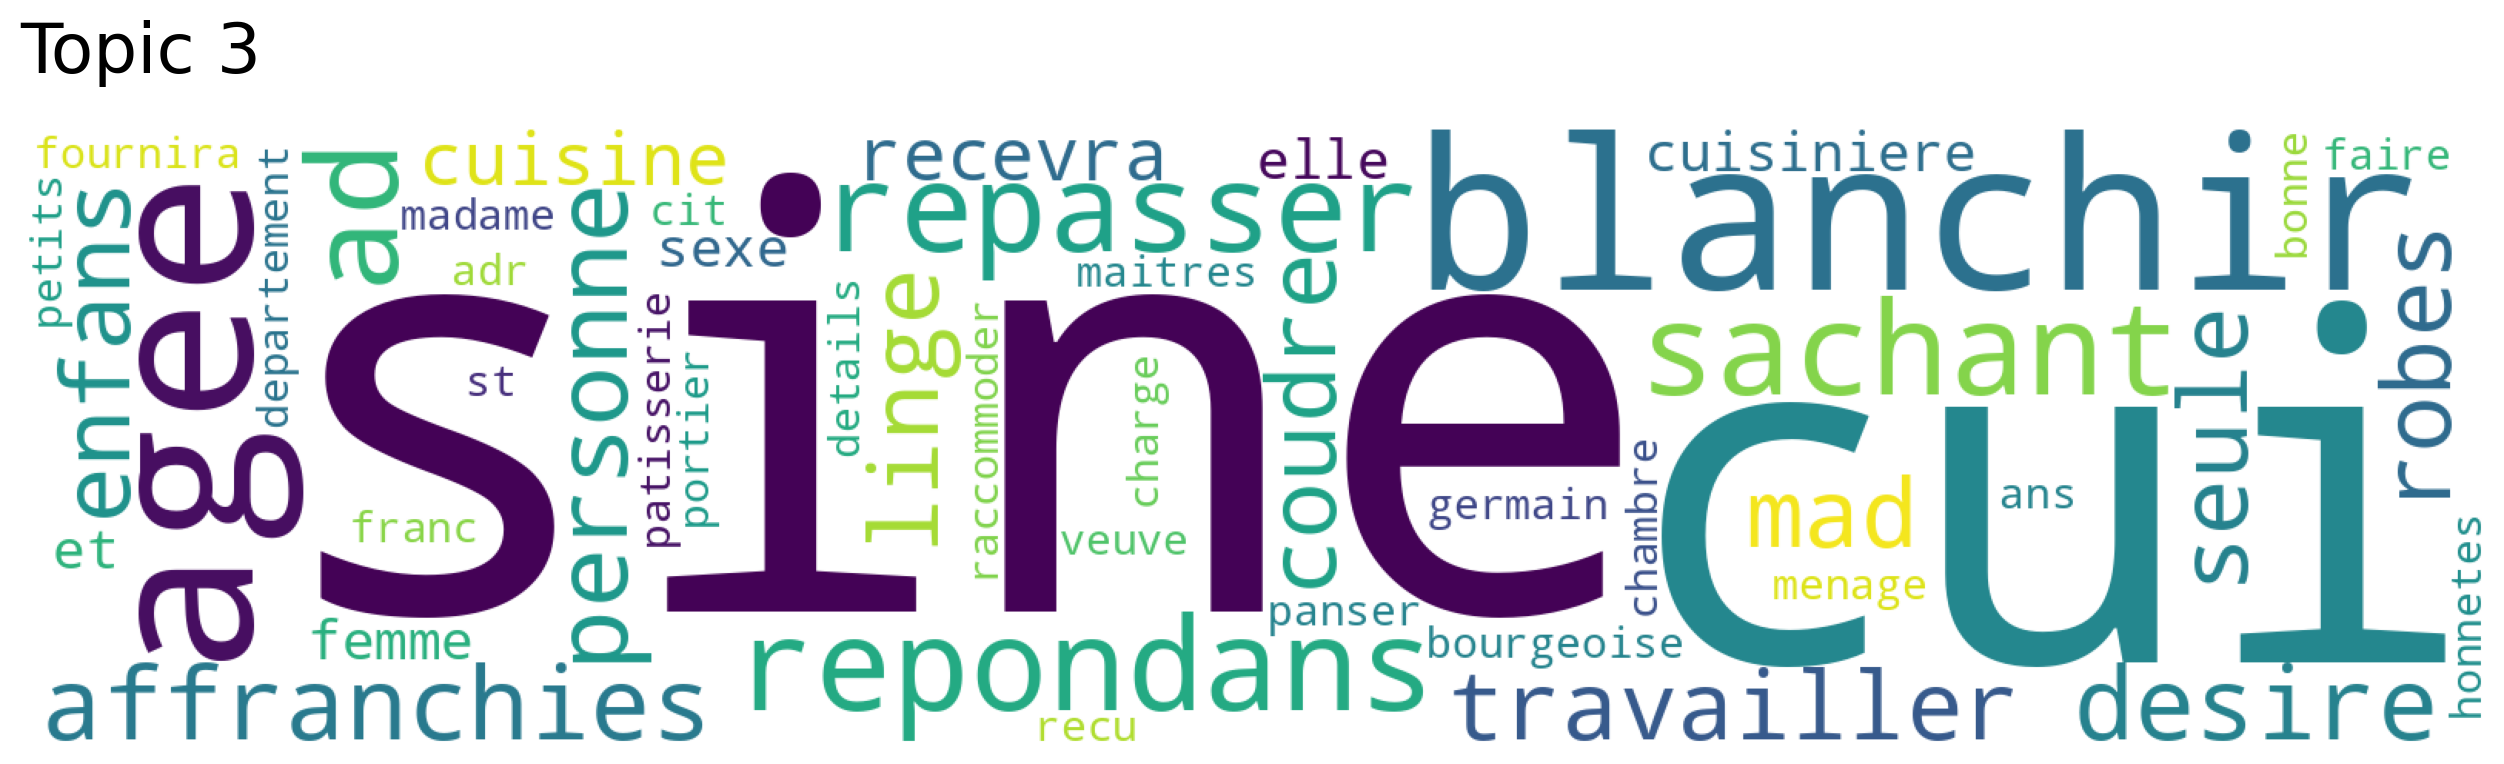
\includegraphics[width=12cm]{wordcloud_top2vec_3.png}
	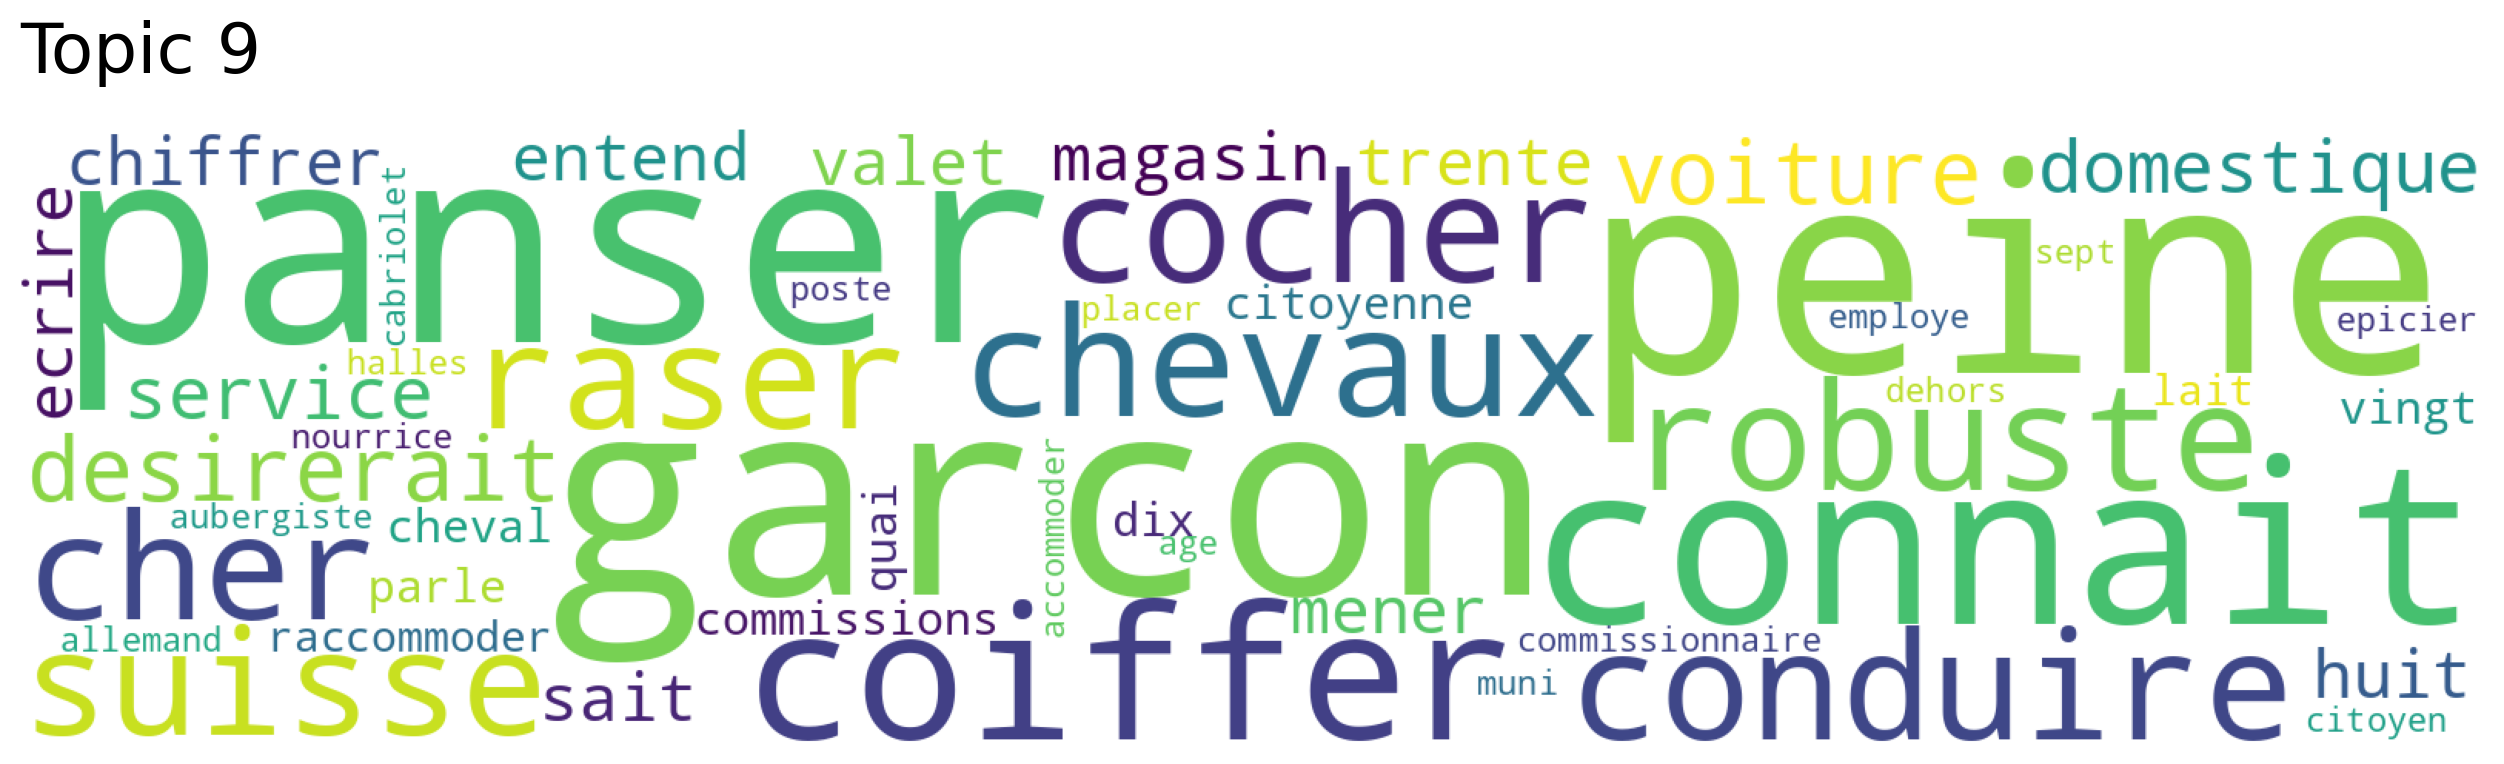
\includegraphics[width=12cm]{wordcloud_top2vec_9.png}
	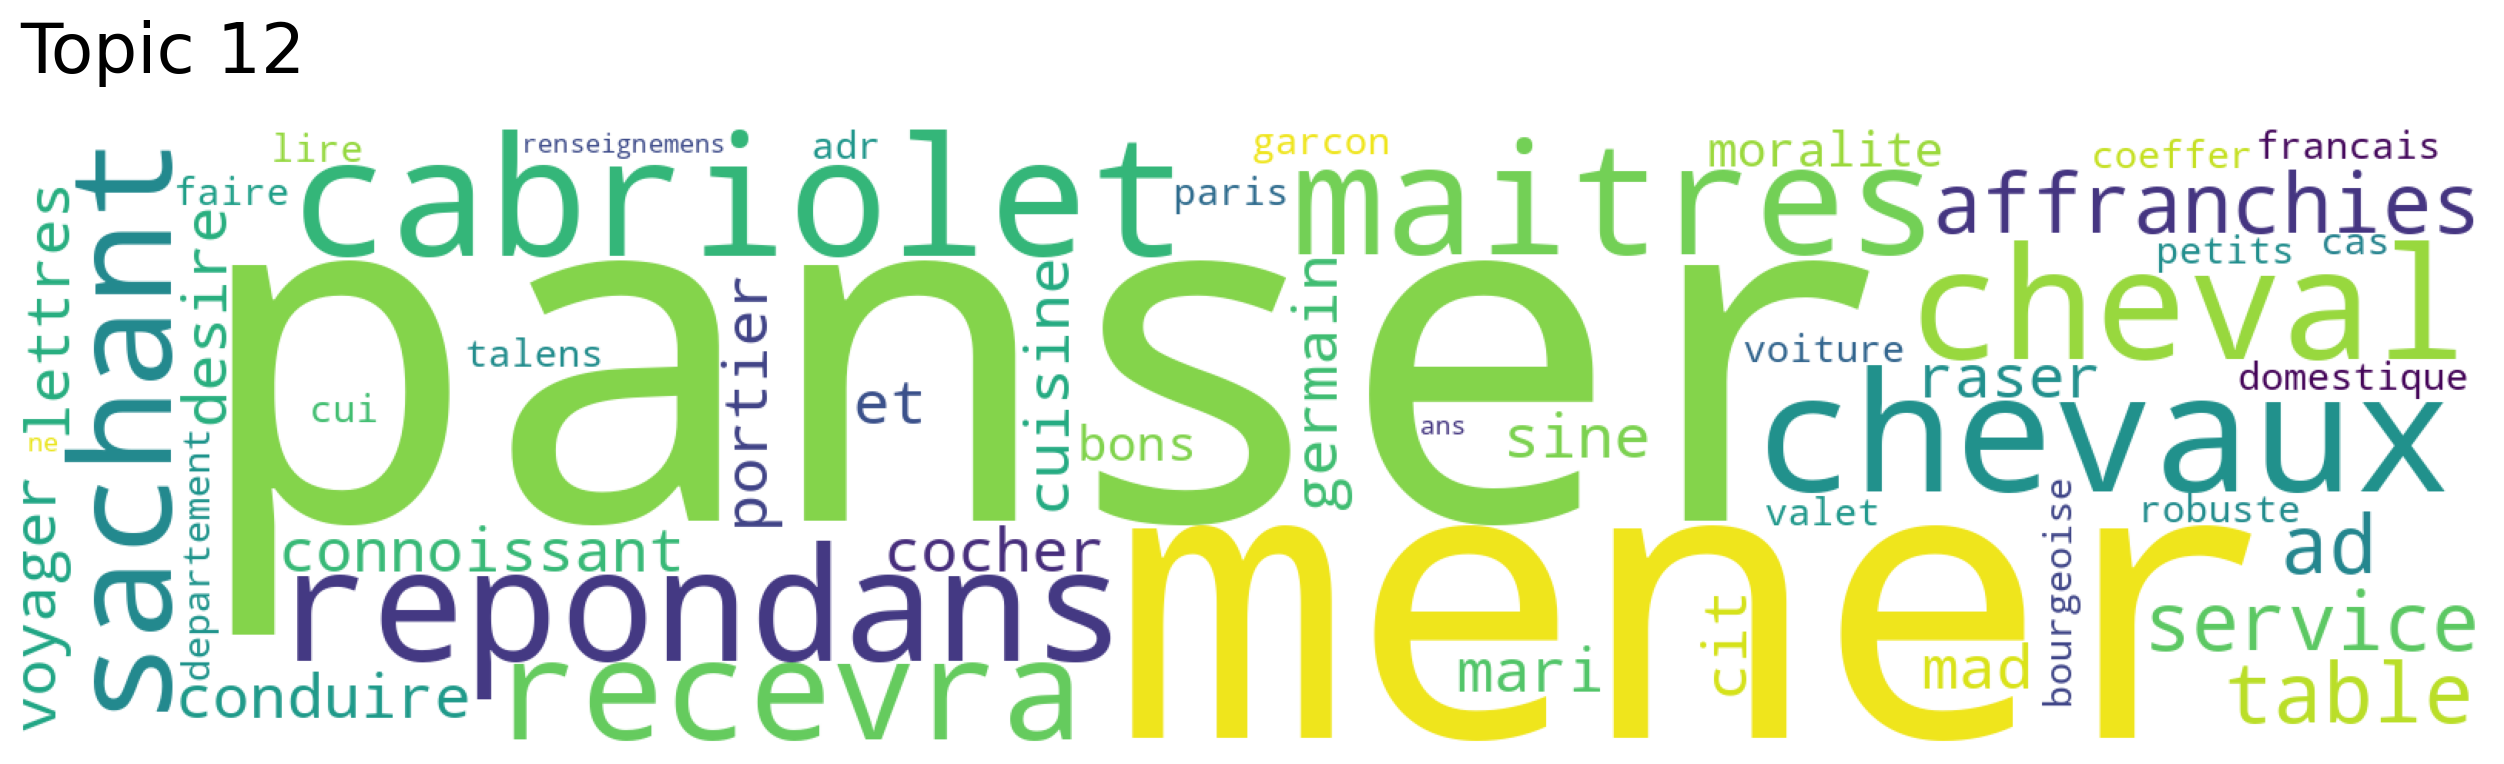
\includegraphics[width=12cm]{wordcloud_top2vec_12.png}
	\caption{Nuage de mots des topics relatifs au genre}
\end{figure}


Par ailleurs, Top2Vec permet également d'interroger la proximité (vectorielle) et donc la similarité (sémantique) des \textit{topics} générés avec d'autres mots, fournis par l'utilisateur, voire même de mots entre eux. Ainsi, les mots les plus similaires (similarité cosine) à "femme" sont, d'après le modèle, "linge" (0.58), "coudre" (0.57), "gouvernante" (0.54), "elle" (0.51) et repasser (0.49). Les mots les plus similaires à "homme" incluent "garçon" (0.48), "conduite" (0.43), "marchand" (0.42) et "affaires" (0.38).

\section{... et révélateurs de la spécificité de la population des annonces}

En plus de confirmer la répartition sexuée du travail au sein des annonces, les\textit{ topics} générés par Top2Vec sont également sensibles à la particularité de certaines annonces, qu'on a déjà étudiées: il s'agit des annonces proposant les services d'une domesticité intellectuelle, qualifiée et spécialisée, parmi lesquels se trouvent précepteurs, secrétaires ou chargés d'affaires. 

Le modèle Top2Vec non seulement les isole des annonces et des compétences plus manuelles, mais divise cette domesticité par spécialisation: le topic 4 est consacré à l'enseignement (histoire, géographie, latine, principes, précepteur); on peut d'ailleurs y percevoir le poids des ecclésiastiques dans l'éducation des jeunes de grande famille. Le topic 6 concerne plutôt le commerce, la gestion des affaires et des terres ou la tenue des comptes (changes, livres, tenir, commerce...), rôle qui incombe généralement au régisseur, au notaire ou à l'homme d'affaires. Enfin, le topic 13, en réunissant les mots "commis", "secrétaire", "plume" et "écriture", semble plutôt désigner les domestiques particuliers du maître, qui sont chargés entre autres de sa correspondance. 

\begin{figure}[h!t]
	\centering
	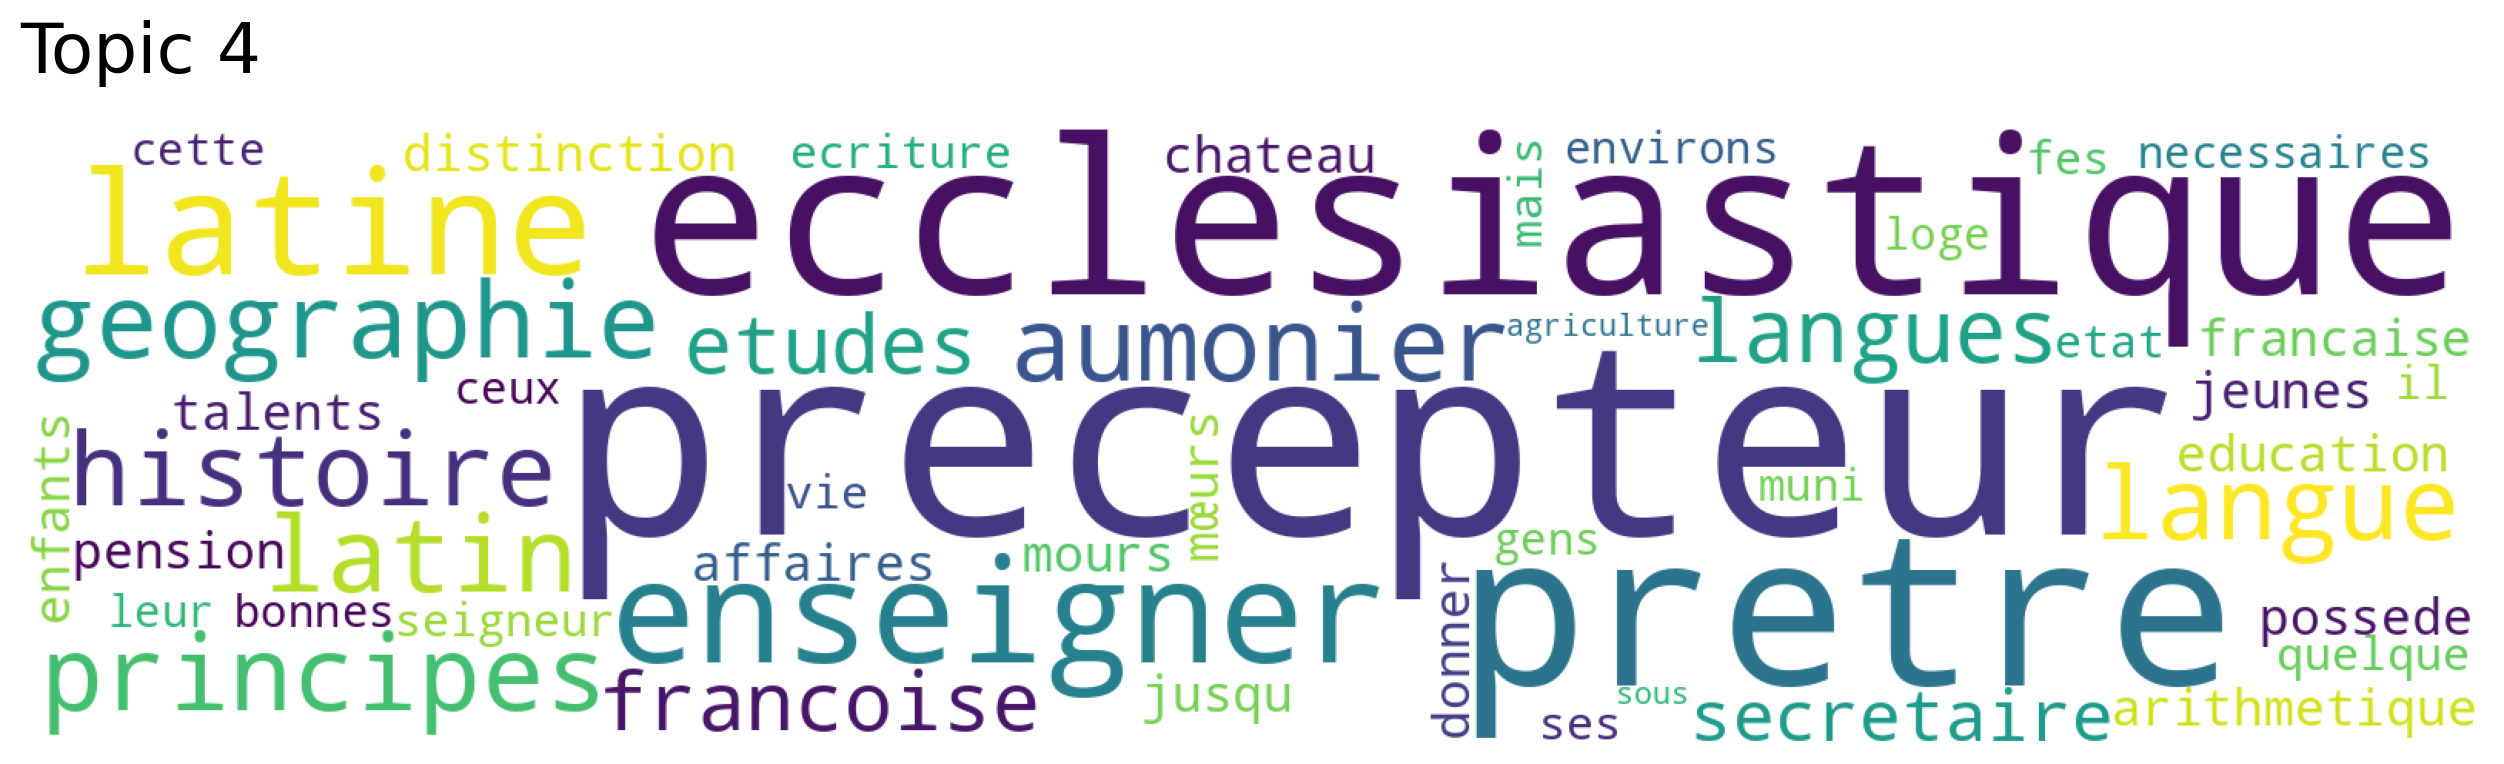
\includegraphics[width=12cm]{wordcloud_top2vec_4.png}
	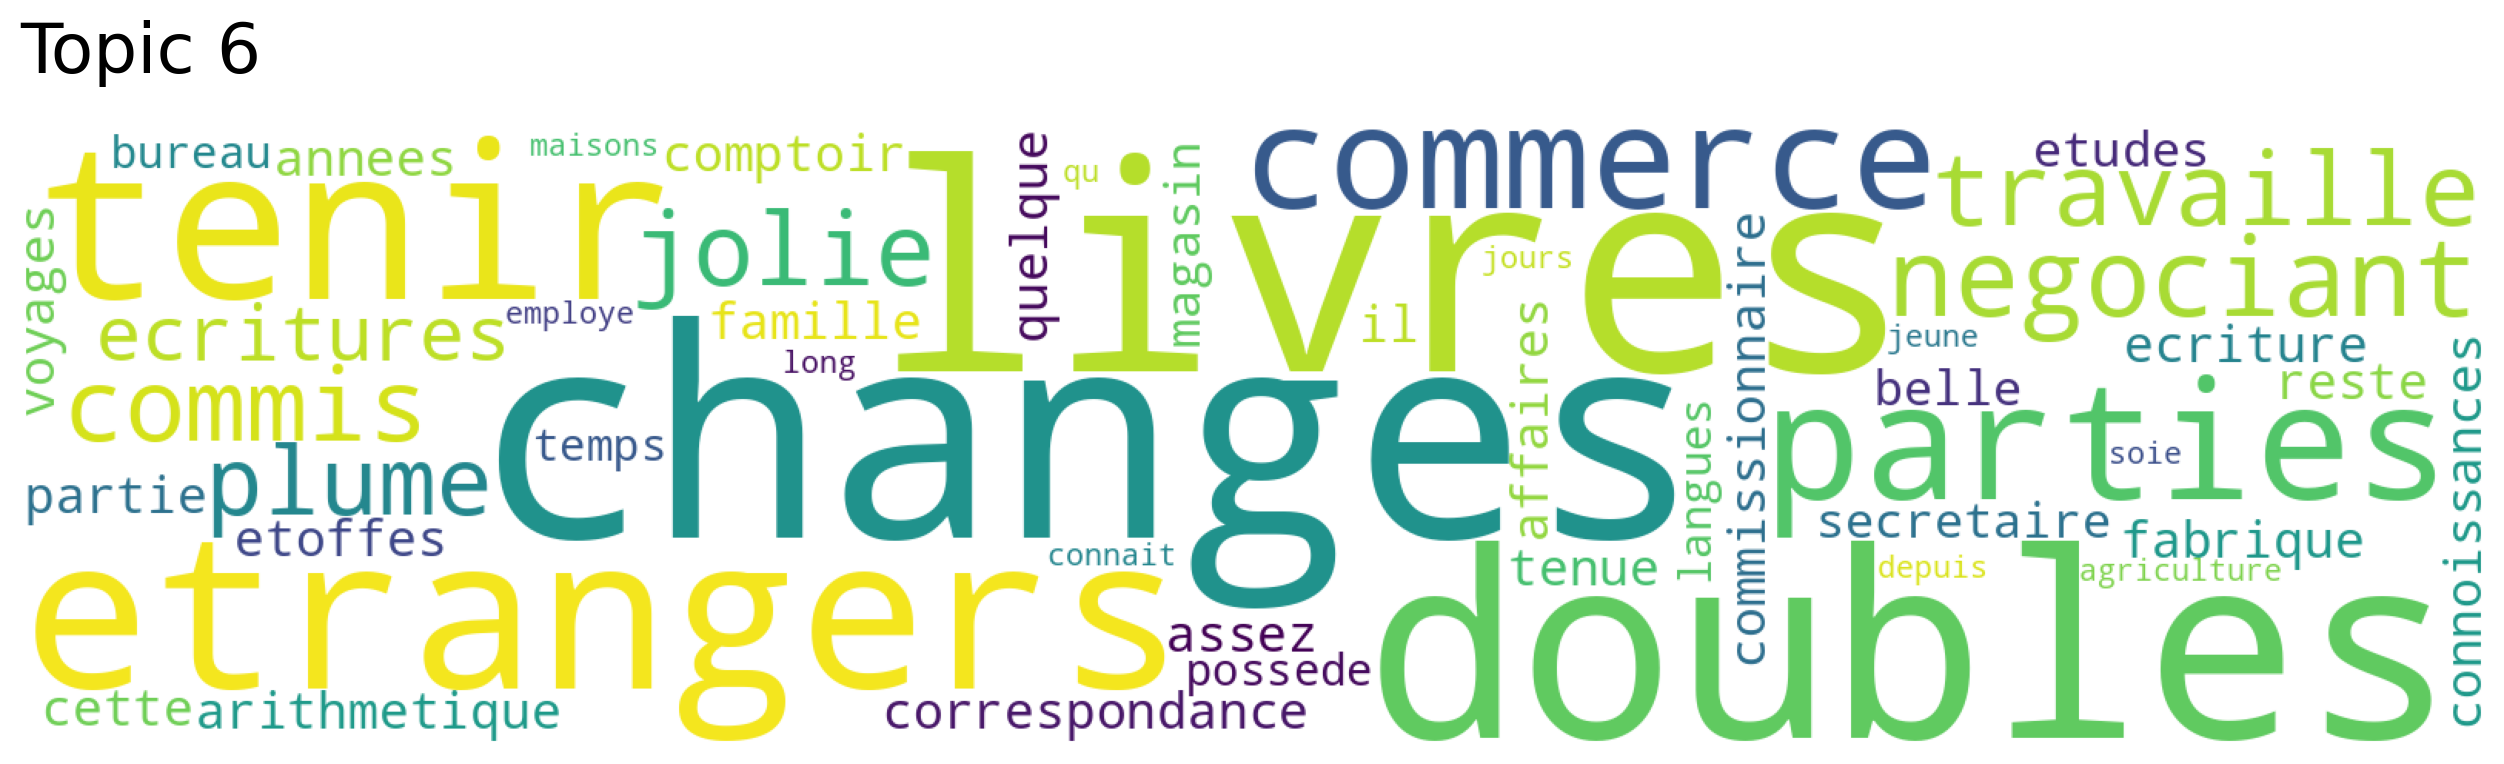
\includegraphics[width=12cm]{wordcloud_top2vec_6.png}
	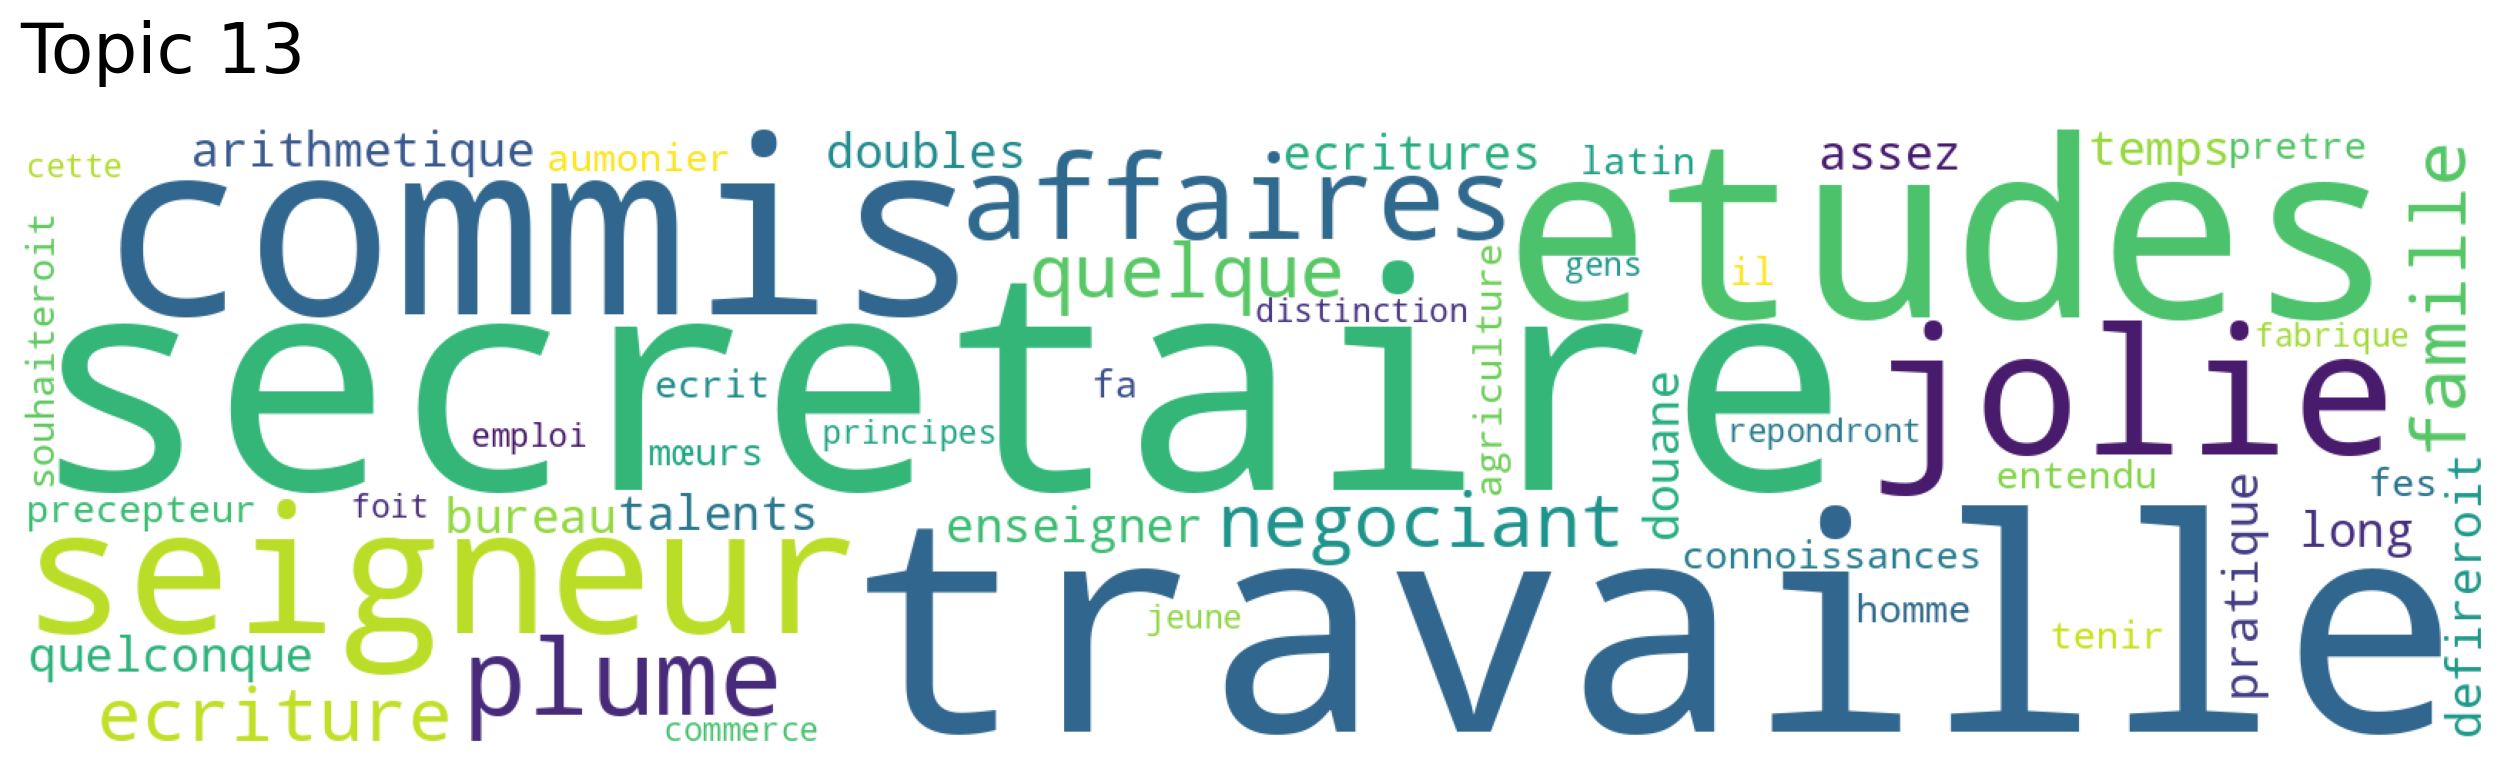
\includegraphics[width=12cm]{wordcloud_top2vec_13.png}
	\caption{Nuage de mots des topics relatifs à la domesticité qualifiée}
\end{figure}

\section{\textit{Topics} et division sociale du travail}

Mais les thèmes générés par le modèle révèlent également un panorama plus large du travail urbain à l'époque moderne, qui rencontre ou recouvre parfois le champ strict de la domesticité. Le topic 10 notamment, dédié au commerce et au travail de boutique (fabrique, étoffes, soie, négociant, fabricant, ...), montre que les annonces déposées ne concernent pas uniquement la domesticité privée; être commis ou fille de boutiques sont également des horizons possibles pour les jeunes gens sans condition. Il s'agit d'un résultat que j'ai eu du mal à déceler avec les méthodes employées jusqu'ici (hormis la présence de "commis" parmi les emplois extraits du corpus) mais qui est révélé grâce au \textit{topic modeling}.

De même, le topic 16 se réfère également au commerce mais lui ajoute cette fois une dimension itinérante (voyages, correspondance), rappel que "les grandes villes agissent comme des plaques tournantes d’un marché du travail dont le périmètre peut transcender le continent européen\footcites{kramplAdresserClercHuissier2017}". 

\begin{figure}[h!t]
	\centering
	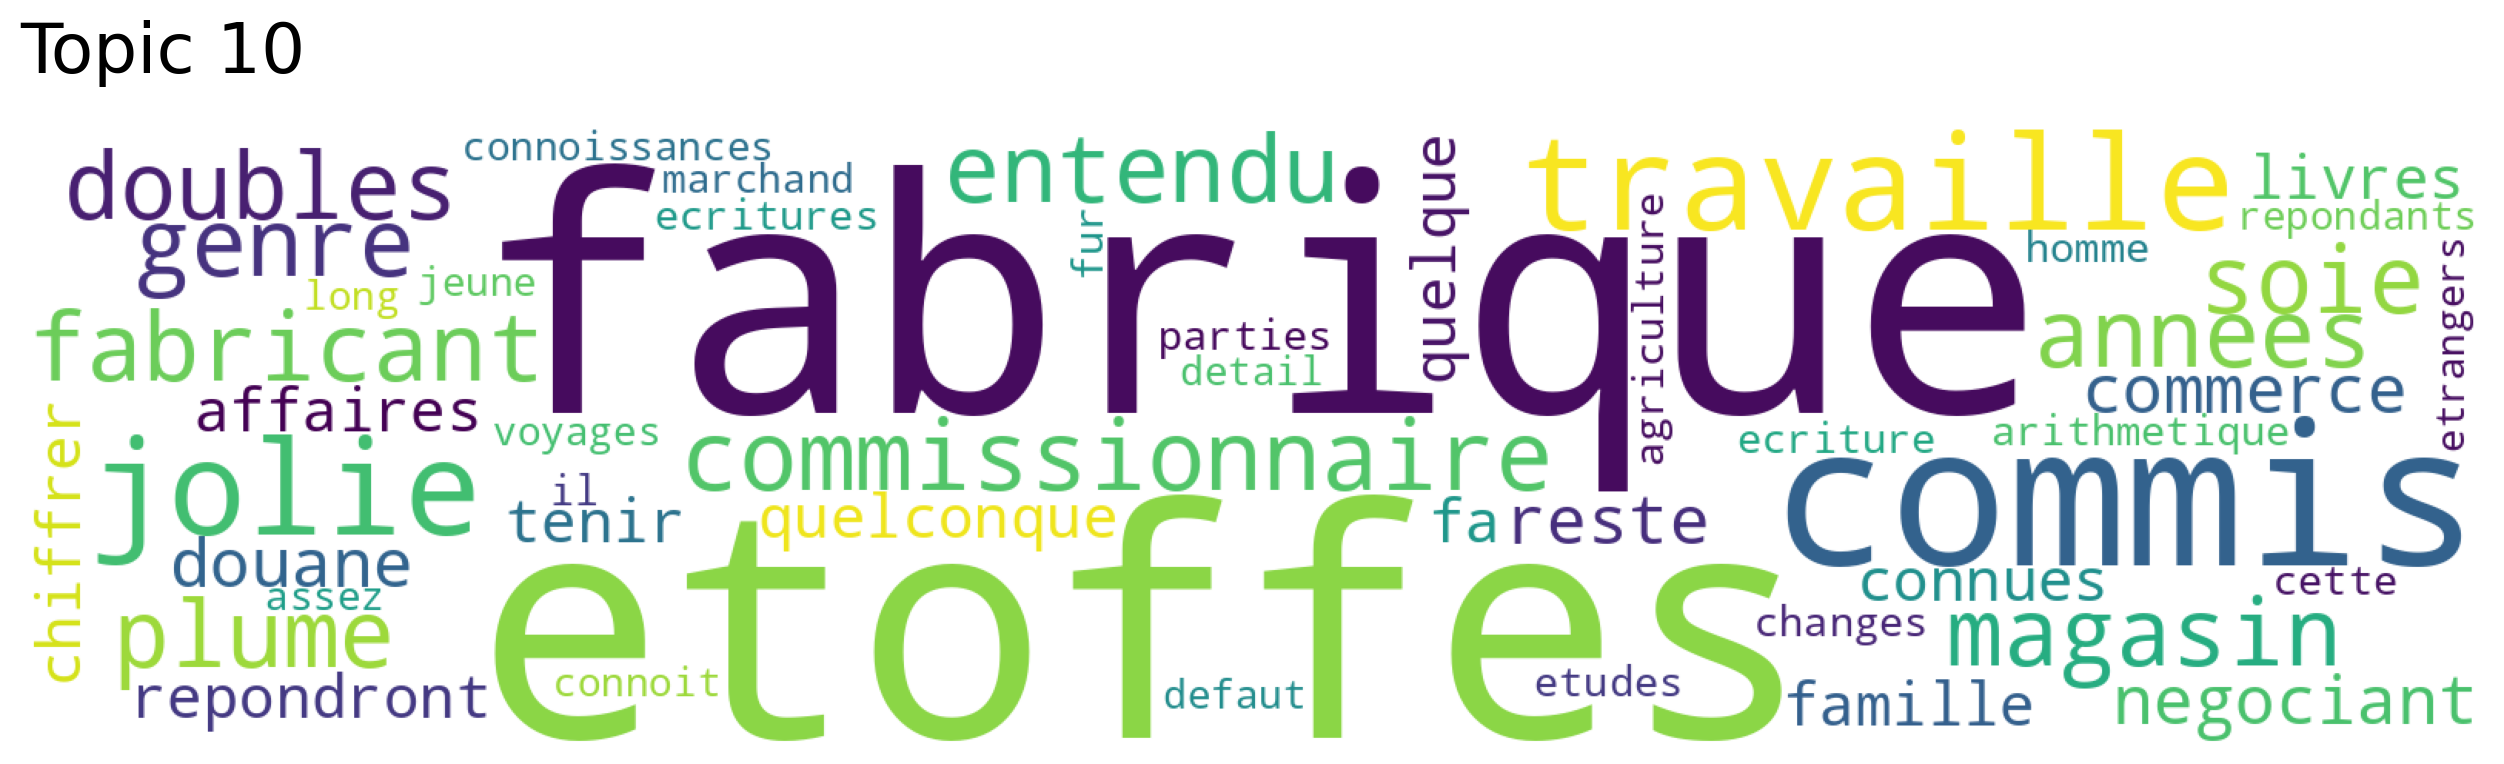
\includegraphics[width=12cm]{wordcloud_top2vec_10.png}
	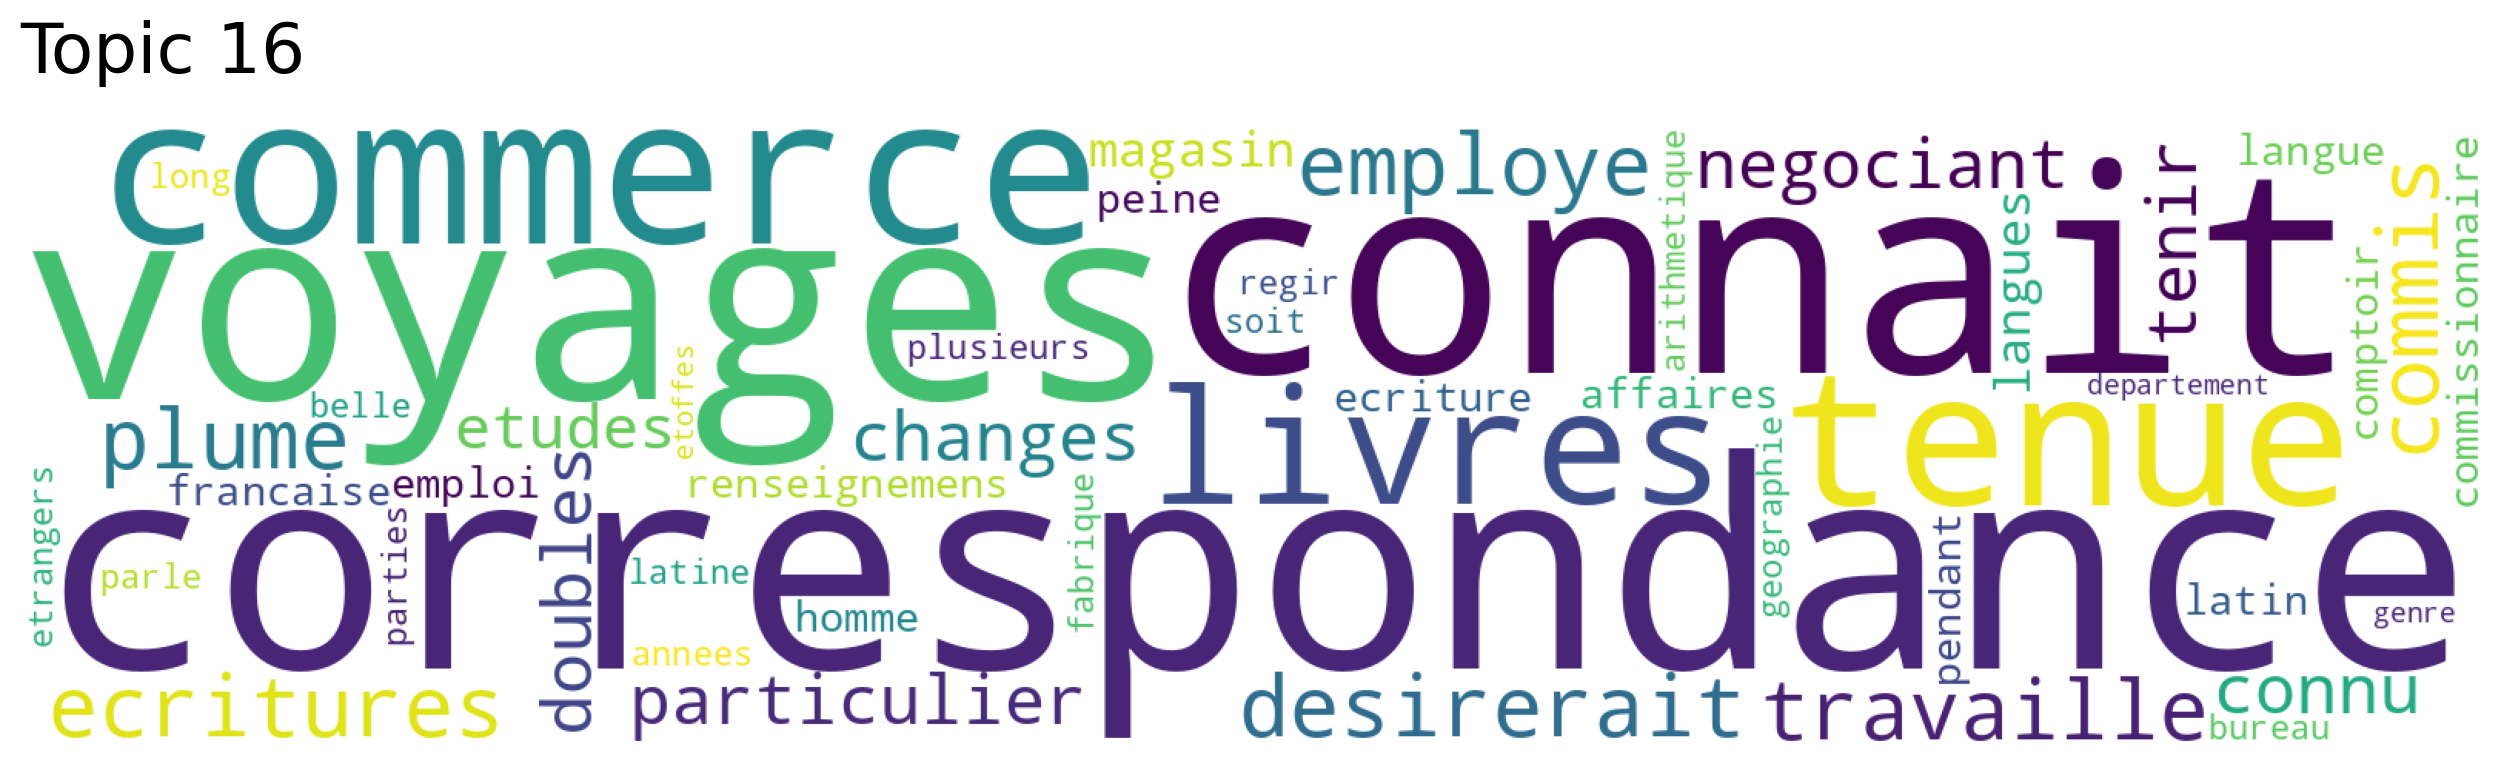
\includegraphics[width=12cm]{wordcloud_top2vec_16.png}
	\caption{Nuage de mots des topics 10 et 16}
\end{figure}

\section{Dévoiler les anomalies du corpus}

Enfin, le \textit{topic modeling}, en associant entre elles les annonces les plus similaires sémantiquement, permet aussi de faire apparaître des anomalies ou des exceptions du corpus, qui seraient autrement passées inaperçues. Ainsi, le topic 5, qui se réfère aux chaises de poste et aux offres de transport (voiture, frais, partir, voyage) est la preuve que ma tentative d'éliminer ces annonces parasites dans le corpus initial a en partie échouée. Ce faisant, le \textit{topic} renseigne indirectement sur l'importance des annonces prenant pour objet le voyage et le "covoiturage"; le journal devient là aussi un support incontournable créant de nouvelles configurations d'intermédiation des personnes\footcites{zellerAuxOriginesCovoiturage2018}. 

\begin{figure}[h!t]
	\centering
	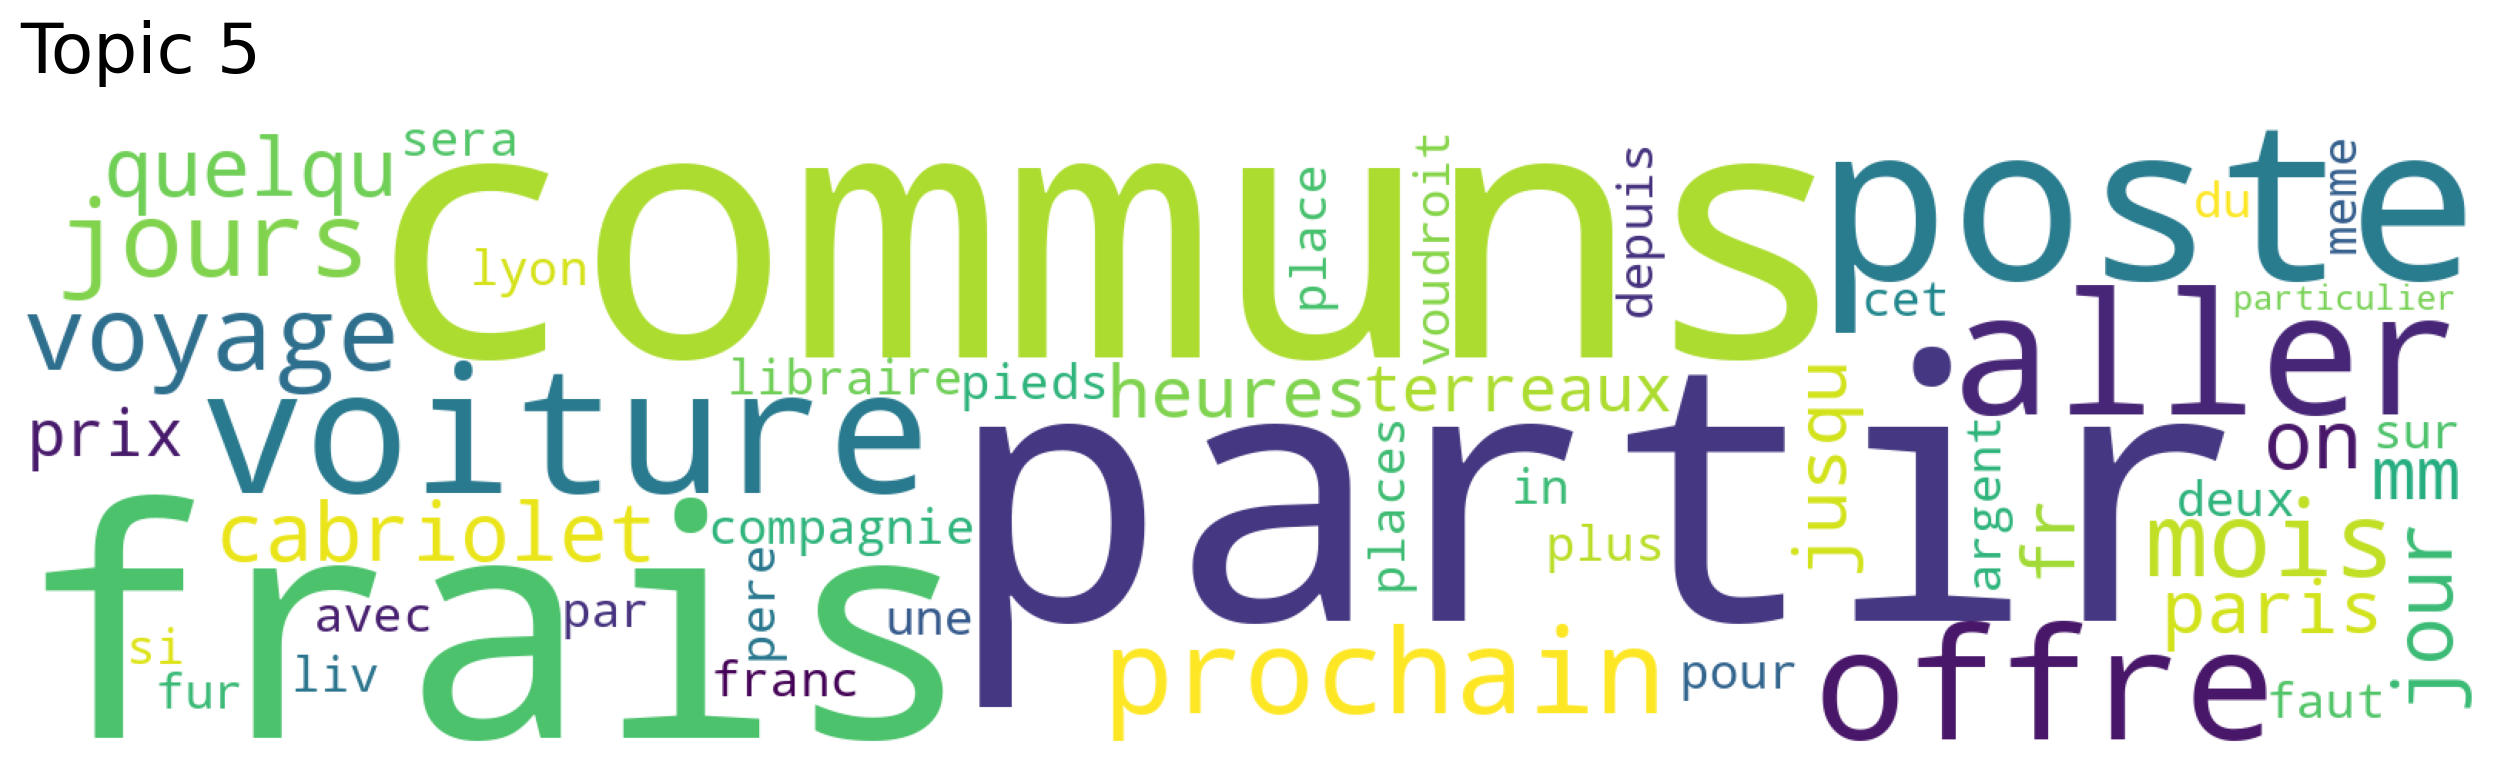
\includegraphics[width=12cm]{wordcloud_top2vec_5.png}
	\caption{Nuage de mots du topic 5}
\end{figure}



\chapter{Modéliser les \textit{topics} dans l'espace social avec BERTopic}

\section{Méthode}

L'algorithme de BERTopic\footnote{Documentation disponible sur le github de BERTopic: \url{https://maartengr.github.io/BERTopic/index.html}}, le troisième et dernier outil de \textit{topic modeling} que j'ai utilisé dans le cadre de cette étude, est par beaucoup d'aspects similaire à celui de Top2Vec: comme lui, il repose sur des \textit{embeddings} et des \textit{clusters} de mots, ne nécessite pas de \textit{pre-processing} des données, procède ensuite à une réduction de dimensionnalité à l'aide de la technique UMAP (\textit{Uniform Manifold Approximation and Projection}), et détermine seul le nombre de \textit{topics} à générer. 

Néanmoins, certaines différences existent entre les deux algorithmes, notamment relatives à la façon dont les clusters sont considérés. Alors que Top2Vec crée des \textit{topics} à partir \textit{clusters} de mots, les mots les plus proches du centre du cluster étant alors les plus représentatifs du topic, BERTopic assemble tous les mots d'un cluster pour en faire un seul document, dont il extrait ensuite les éléments les plus représentatifs à l'aide d'une mesure Tf-Idf (\textit{Term Frequency - Inverse Document Frequency}. Les termes les plus pertinents sont donc ceux qui auront le plus grand nombre d'occurrences dans un document (\textit{Term Frequency}), rapportés à leur rareté relative dans le corpus (\textit{Inverse Document Frequency}). Ainsi, des mots très courants dans l'ensemble des documents du corpus (les mots-vides, par exemple) ont peu de chances d'être considérés comme pertinents; en revanche, un mot rare à l'échelle du corpus, mais présent plusieurs fois dans un même document, a beaucoup de chances d'être sélectionné. 

Par ailleurs, BERTopic permet, contrairement à Gensim ou Top2Vec, de concaténer les \textit{topics} par classe (dans notre cas, par ville par exemple) et de réaliser un \textit{topic modeling} dynamique, permettant de visualiser les évolutions du poids des \textit{topics} dans le temps. Pour mobiliser ces deux possibilités offertes par l'algorithme, j'ai au préalable créé deux nouveaux \textit{datasets} plus équilibrés, le premier en sélectionnant aléatoirement mille annonces de chaque ville (au total, 3000 annonces), et le second en sélectionnant cent annonces pour chaque année de publication (au total, 3900 annonces). 

\section{Aperçu général des \textit{topics}: beaucoup de similarités avec Top2Vec, quelques différences}


Le modèle généré à partir du corpus d'origine a permis de distinguer vingt-quatre \textit{topics}, soit autant qu'avec Top2Vec. Parmi ceux-ci, on observe beaucoup de \textit{topics} semblables à ceux générés par le premier algorithme: certains centrés sur le travail féminin (topic 0), d'autres plutôt sur la domesticité masculine (topics 3, 5, 18, 20, 22) ou qualifiée (topics 1, 6, 7, 13, 17). La présence du commerce semble plus importante qu'avec Top2Vec, où elle ne représentait que deux \textit{topics} sur 24; ici, on retrouve la vente et la description des marchandises dans le \textit{topic} 10, le marché très spécifique du vin avec le \textit{topic} 16, et les emplois et intermédiaires du monde marchand (commissionnaires) dans le \textit{topic} 23. 

La matrice de similarité générée par le modèle, permet également d'observer les proximités sémantiques entre topics, qui souvent sont signifiantes de proximités socio-démographiques (les \textit{topics} 5 et 9 par exemple, qui ont un score de similarité supérieur à 0.9, concernent respectivement le service personnel du maître et l'emploi domestique dans le monde marchand, mais ils ont la particularité de tous deux contenir des qualifiatifs masculins, notamment "garçon") ou de proximités sur le marché du travail (les \textit{topics} 13 et 21, qui ont un score de similarité de 0.91, concernent tous les deux les emplois de boutiques). 

\begin{figure}[h!t]
	\centering
	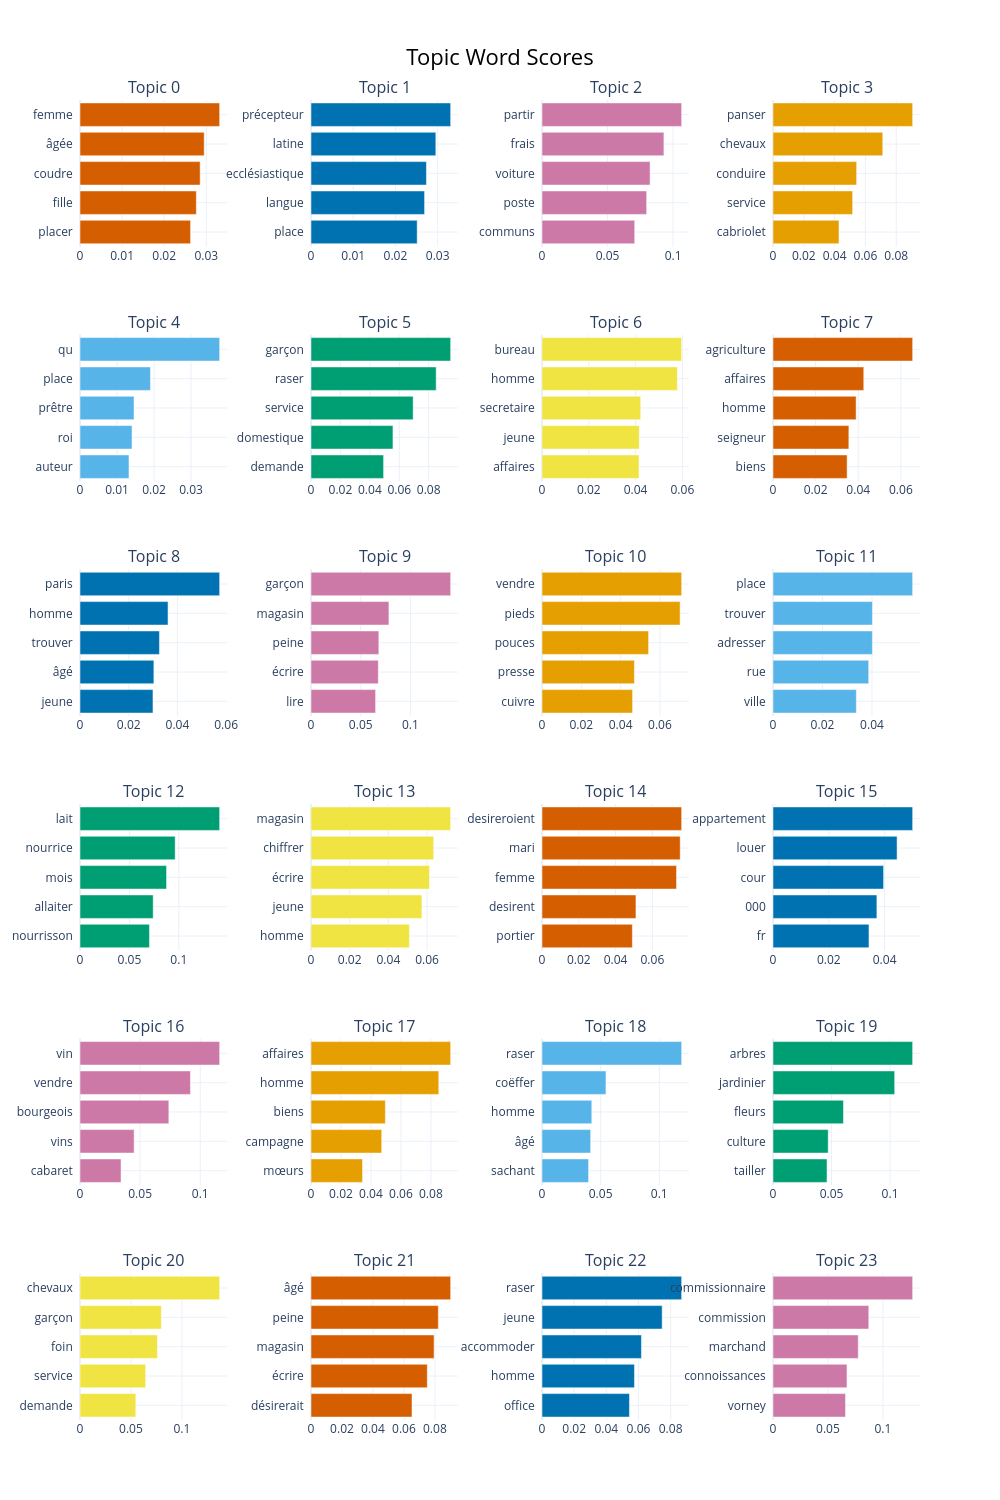
\includegraphics[width=15cm]{plot_bertopic.png}
	\caption{Vingt-quatre \textit{topics} générés par BERTopic}
\end{figure}

\begin{figure}[h!t]
	\centering
	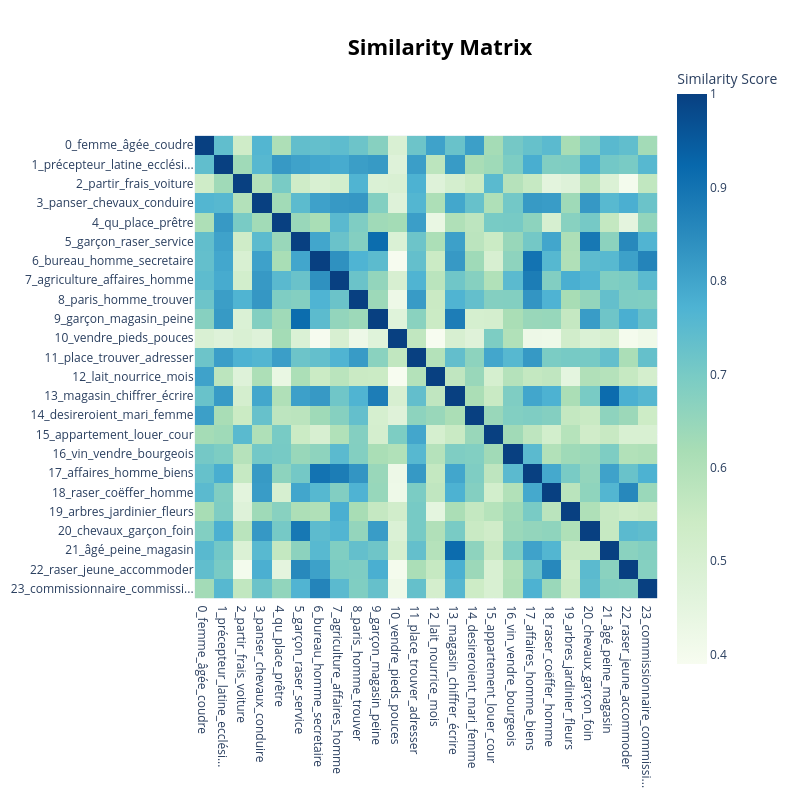
\includegraphics[width=12cm]{matrice_bertopic.png}
	\caption{Matrice de similarité entre les \textit{topics} générés par BERTopic}
\end{figure}



Deux \textit{topics}, cependant, révélateurs de segments très particuliers du marché du travail, n'apparaissent qu'avec BERTopic. Il s'agit tout d'abord du \textit{topic} 12, dédié aux nourrices en recherche d'emploi, que je n'ai pas pu traiter dans le cadre de ce travail en raison de leur très faible présence dans les \textit{Affiches} (moins de 50 occurrences). Néanmoins, il ne parait pas étonnant que le modèle parvienne à différencier les annonces de nourrices du reste des annonces d'emploi, tant le vocabulaire et les formules qui y sont employées diffèrent du reste du corpus: ici, pas (ou peu) de mention de compétences manuelles ou de connaissances de certaines langues, les informations données ont principalement trait à la santé de la nourrice, à la qualité et à l'âge de son lait. Par exemple, cette annonce lyonnaise en date du 15 décembre 1803, où "une jeune Veuve qui jouit de la meilleure santé, et dont le lait a vingt mois, [désire] trouver un Nourrisson pour l'allaiter chez elle\footnote{\textit{Affiches de Lyon}, 15 décembre 1803}", est très représentative.

Le second \textit{topic} unique à BERTopic est le \textit{topic} 19, consacré aux annonces de jardiniers. Rattaché à la domesticité spécialisée et de plus en plus demandée au XVIIIè siècle avec l'avènement des jardins urbains\footcites{synowieckiParisSesJardins2021}, le jardinier se distingue des autres domestiques qualifiés en ce qu'il n'exerce pas une activité à proprement dit intellectuelle. Cette différence se ressent dans les mots employés dans les annonces, qui relèvent de compétences artistiques mais surtout physiques (tailler) et doivent également signifier les connaissances précises et quasi-scientifiques acquises par le domestique dans son domaine (connaissance des différentes cultures, des soins des fleurs comme des arbres). Sa présence comme \textit{topic} distinct n'est donc pas étonnante tant sa recherche d'emploi se distingue de celle des autres serviteurs, par son exercice à l'extérieur du foyer autant que par son caractère pluriel, à la fois manuel et très spécialisé. 




\section{Resituer les \textit{topics} géographiquement et chronologiquement}

\subsection{Le \textit{topic modeling} par ville}

Enfin, j'ai décidé de conclure cette incursion dans les annonces en tirant parti de deux fonctionnalités fournies par BERTopic: le \textit{topic modeling} par classe et le \textit{topic modeling} roulant, ou dynamique. Pour ces deux analyses, j'ai dû, face aux déséquilibres du corpus initial (surreprésentation de Lyon et du début du XIXè siècle notamment), créer des jeux de données spécifiques. Les \textit{topics} présentés ne seront donc pas les mêmes que ceux de la partie précédente, et le mode de constitution des nouveaux corpus (par sélection aléatoire, avec doublons dans le cas où les annonces manqueraient, comme pour Bordeaux) appelle à la prudence. 

\begin{figure}[h!t]
	\centering
	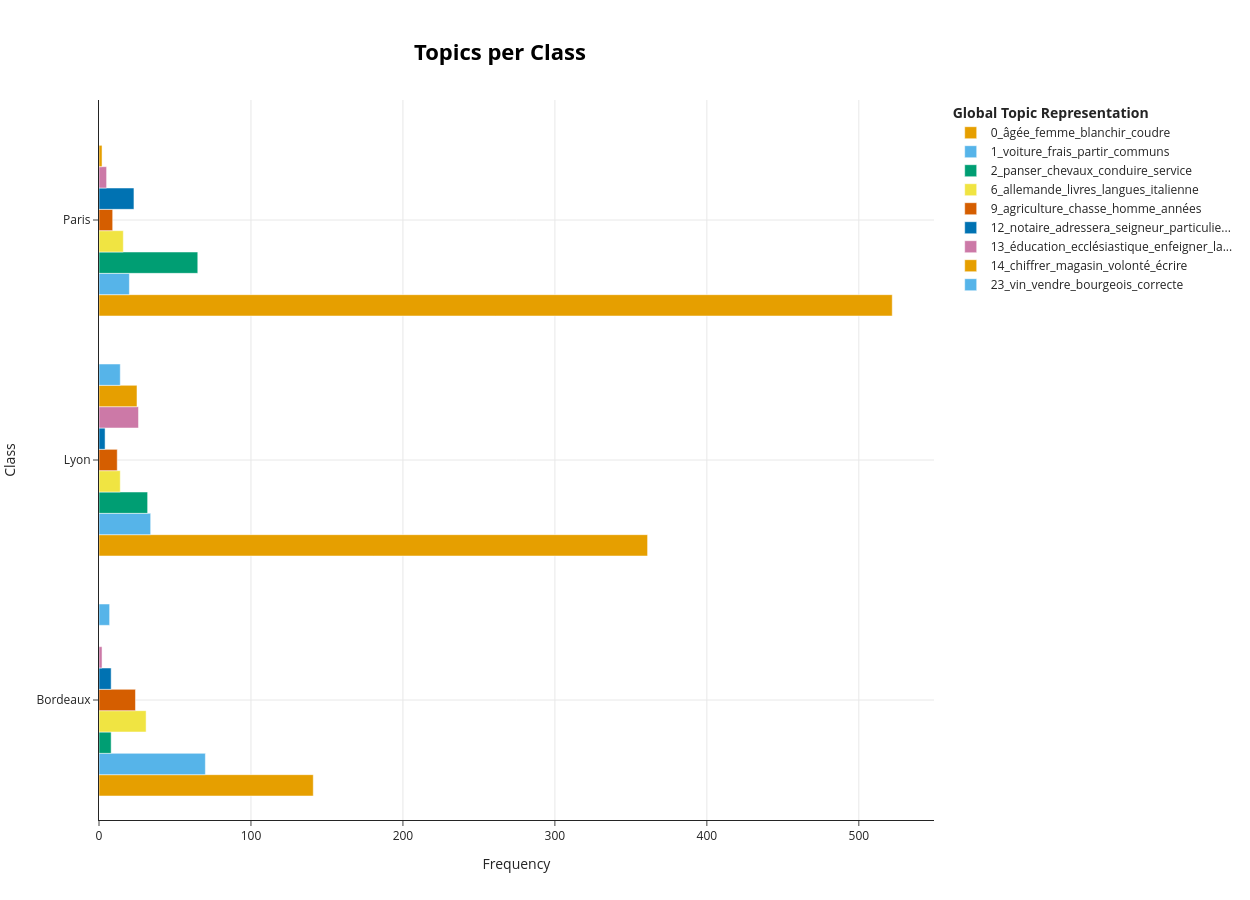
\includegraphics[width=15cm]{bertopic_villes.png}
	\caption{Résultat du \textit{topic modeling} par ville avec BERTopic}
\end{figure}

Les graphique obtenu permet ainsi de mesurer le poids de chaque ville dans la génération des topics: si Paris est surreprésenté parmi les annonces d'emplois domestiques manuels (\textit{topics} 0 "femme, blanchir, coudre" et 2 "panser, chevaux, conduire"), Bordeaux et Lyon semblent plus concernées par la domesticité qualifiée (\textit{topics} 6, 13 et 14) ainsi que le commerce de vin (\textit{topic} 23).

\subsection{Le\textit{ topic modeling} roulant dans le temps}

Quant à lui, le \textit{topic modeling }roulant, s'il s'annonçait prometteur pour capter les évolutions du marché de l'emploi domestique sur la période étudiée, semble malheureusement trop dépendant des lacunes du corpus, et ce malgré le rééquilibrage effectué. L'intervalle 1783-1795, pour lequel aucun numéro n'est disponible, rend difficile l'interprétation des données restantes. Tous les \textit{topics} ou presque semblent connaître des variations entre 1750 et 1805, mais celles-ci semblent plus liées aux variations internes au corpus.


\begin{figure}[h!t]
	\centering
	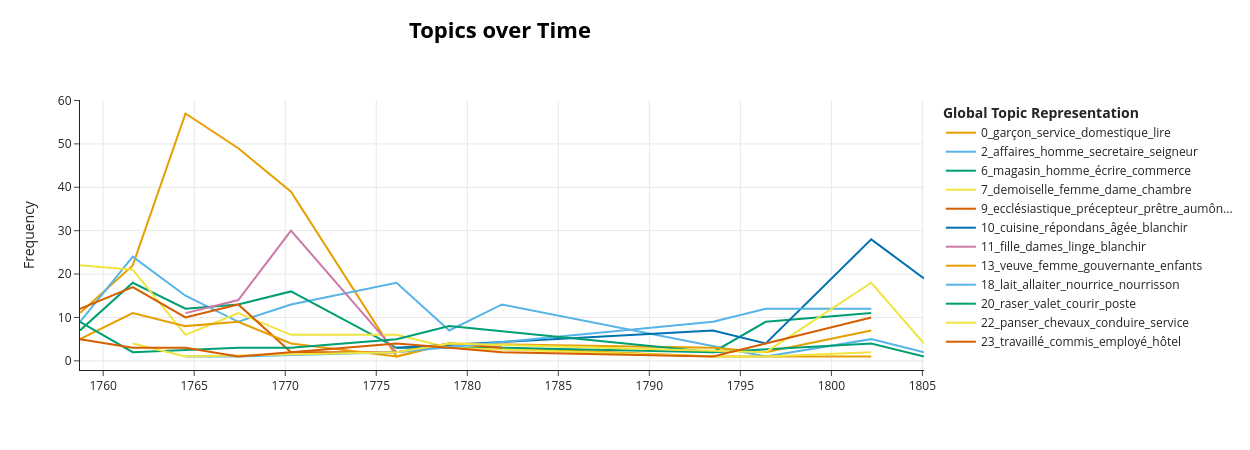
\includegraphics[width=15cm]{bertopic_temps.png}
	\caption{Résultat du \textit{topic modeling} dynamique avec BERTopic}
\end{figure}